% !Mode:: "TeX:UTF-8"
\chapter{Подход построения нацеленных тестов, сопутствующие ему методы и модели}

\section{Метод построения нацеленных тестов}
Основные шаги следующие:
\begin{enumerate}
  \item чтение документации по архитектуре;
  \item выделение интересных для тестирования ситуаций;
  \item формализация архитектуры;
  \item подготовка конструктора инициализирующей программы;
  \item запуск генератора для каждой ситуации.
\end{enumerate}

То есть предлагаемый метод следует подходу нацеленной генерации тестов. Для
тестируемого микропроцессора всегда есть описание его архитектуры. В этом
документе, фактически, описано, как должны действовать, функционировать, разные
инструкции. Разработчики тестов сначала размечают эти описания -- выделяют
разные случаи исполнения инструкций. Затем на основе выделенных случаев строится
шаблон теста, который исходит из идей разработчиков тестов, в какие ситуации
надо попасть при исполнении инструкций. Затем для возможности автоматического
построения тестов выделенные случаи исполнения инструкций формализуются.
Специальный генератор на основе этого формального описания будет строить для
шаблона инструкции теста и инициализацию микропроцессора.
Для выражения этой инициализации в виде инструкций надо написать конструктор
инициализирующей программы.

\begin{figure}[p] \center
  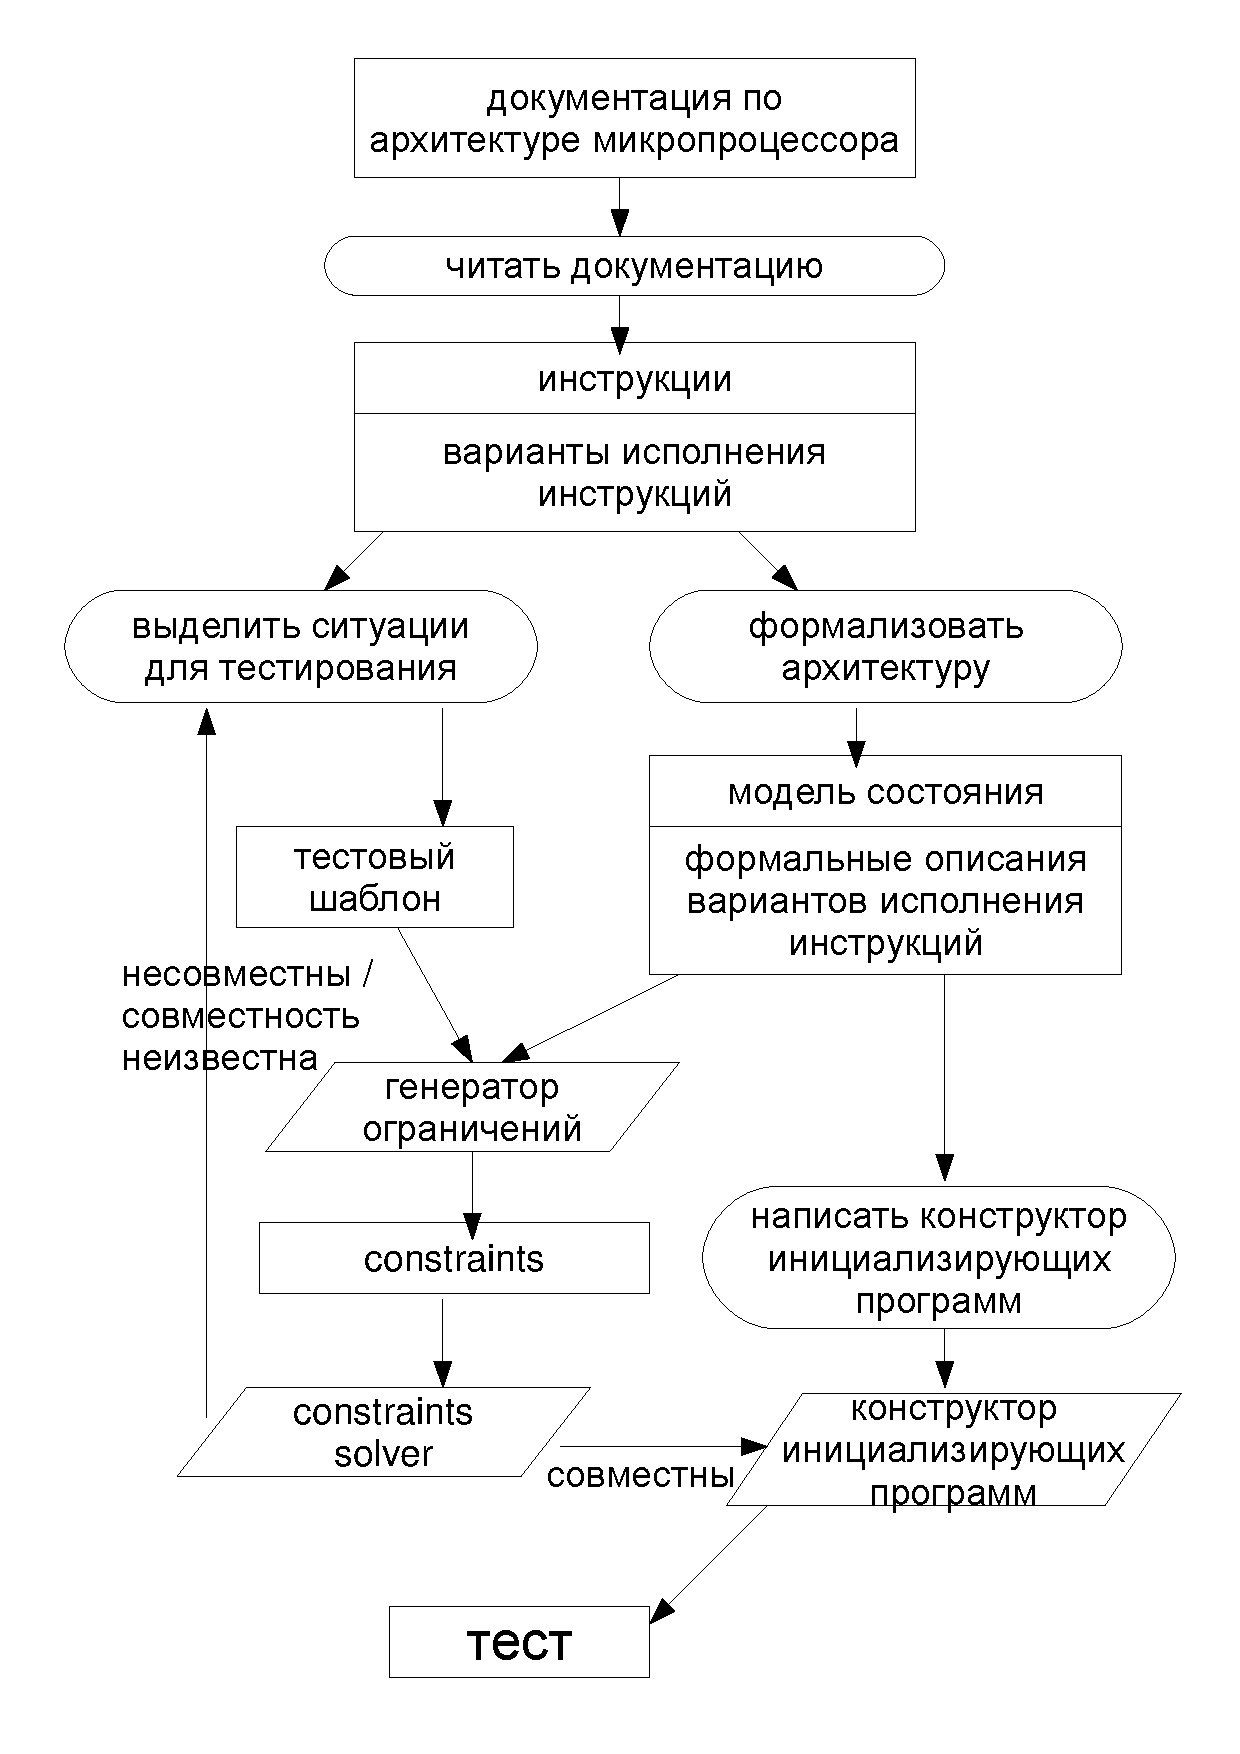
\includegraphics[width=0.9\textwidth]{2.theor/process_full}\\
  \caption{Предлагаемый метод генерации тестов}\label{process}
\end{figure}

Предлагаемый метод с указанием потоков данных изображен на
рисунке~\ref{process}. Действия, которые надо выполнить вручную, помещены в
прямоугольники с закругленными краями. Данные помещены в прямоугольники.
Программные компоненты помещены в параллелепипеды~\cite{my_lomonosov_2009, my_miet_2009}.

Теперь более подробно будут описаны шаги предлагаемого метода.

\paragraph{шаг <<читать документацию>>} <<Документация по архитектуре>> --- это
документ, описывающий семантику инструкций микропроцессора и некоторые
структурные характеристики микропроцессора (какие есть разные буферы, кэш-память
и др).
В результате чтения документации надо:
\begin{enumerate}
  \item выделить инструкции, их формат (какие возможны аргументы);
  \item выделить в инструкциях варианты исполнения (<<разметить>>, обычно один
вариант исполнения описывается в виде последовательности более простых
действий), каждому варианту исполнения присвоить идентификатор (метку);
  \item определить для каждого варианта исполнения, в какие блоки
микропроцессора происходят в нем обращения (кэш-память некоторых уровней, буфер
трансляции адресов и т.п.).
\end{enumerate}

Например, документация по архитектуре MIPS64 описывает инструкцию LW загрузки
32х бит из памяти в регистр; эта инструкция обладает следующими вариантами
исполнения (приведены лишь некоторые из них):
\begin{itemize}
    \item возникновение исключения по причине невыровненного виртуального
адреса;
    \item неотображаемое исполнение --- в котором физический адрес вычисляется
по виртуальному без обращений к каким-либо блокам микропроцессора;
    \item некэшируемое исполнение --- в котором обращение в кэш-память не
делается, напрямую идет обращение в оперативную память;
\end{itemize}

На данном шаге описание варианта исполнения этой инструкции может быть таким: 1)
вычисляется виртуальный адрес --- сумма аргументов, 2) если <<виртуальный адрес
отображаемый>>, вычисляется номер виртуальной страницы, для нее в TLB ищется
соответствующая страница физической памяти (<<идет обращение в TLB>>), иначе
вычисляется физический адрес как битовая подстрока виртуального адреса и т.д.

\paragraph{шаг <<выделение ситуаций для тестирования>>} предполагает составление
<<тестовых шаблонов>>. Напомню, что тестовый шаблон фиксирует интересную для
тестирования ситуацию. Ситуация задается вариантами исполнения инструкций и
цепочками инструкций. Тем самым шаблоны представляют собой последовательности
инструкций с аргументами. Возможно, аргументы в разных инструкциях повторяются.
И у каждой инструкции указывается набор идентификаторов, обозначающих вариант
исполнения инструкции.

Для тестового шаблона будет строиться тест, в котором инструкции будут исполнены
согласно указанным вариантам исполнения. Каждый тест будет состоять из двух
частей: вторая часть --- это те же инструкции и аргументы, что были в шаблоне, а
первая часть (т.н. \emph{инициализирующая программа}) это тоже набор инструкций,
которые подготавливают модель микропроцессора к выполнению инструкций шаблона в
заданных вариантах исполнения инструкций.

\begin{figure}[h]
\quad\parbox{0.5\textwidth}{ \tt
LW x, y, c @ l1Hit } \parbox{0.3\textwidth}{ \tt
XOR y, y, y\\
SW x, y, 0x0\\
LW x, y, 0x0\\}
\caption{Тестовый шаблон (слева) и один из возможных тестов для него
(справа)}\label{test_template_exmp1}
\end{figure}

Пример шаблона и соответствующего ему теста приведен на
рисунке~\ref{test_template_exmp1}. Инструкция LW --- инструкция загрузки 32х бит
из памяти, XOR --- инструкция исключающего ИЛИ, SW --- инструкция сохранения 32х
бит в памяти. Идентификатором \texttt{l1Hit} было помечено исполнение инструкции
LW без трансляции адреса, но с обращением в кэш-память первого уровня с
кэш-попаданием в нем. В тесте, во-первых, выбрано значение константы <<c>>
(равно 0) и, во-вторых, перед инструкцией LW вставлена инструкция SW с теми же
аргументами, что и у LW для того, чтобы данные по этому адресу точно попали в
кэш-память первого уровня и при исполнении инструкции LW в кэш-памяти первого
уровня произошло кэш-попадание.

\paragraph{шаг <<формализовать архитектуру>>} предполагает построение модели
состояния микропроцессора и подготовку формальных описаний вариантов исполнения
инструкций (формализовать <<идентификаторы>>, обозначающие варианты исполнения
инструкций). Состояние образуют те блоки микропроцессора, к которым обращаются
инструкции тестового шаблона. Это могут быть разные регистры, кэш-память разных
уровней, буферы трансляции адресов, вспомогательные буферы. Все они обладают
состоянием (поскольку в них хранятся и изменяются данные).

Формализация архитектуры нацелена на детализацию описания поведения инструкции с
возможностью автоматического построения теста. Формализация выполняется на
основе выделенных на первом шаге описаний вариантов исполнения инструкций. Они
хотя и не всегда формальные, но зачастую высоко формализованы. Формализованное
описание варианта исполнения инструкции представляет из себя последовательность
операторов на специальном языке (ниже этот язык и механизмы, которые он
предоставляет, будут описаны подробнее).

Рассмотрим пример того, как получается формальное описание варианта исполнения
l1Hit инструкции LW архитектуры MIPS64. Формат этой инструкции следующий:
\begin{verbatim}
LW rt, offset(base)
\end{verbatim}

Описание этой инструкции в документации выглядит следующим образом:
\begin{verbatim}
  vAddr <- sign_extend(offset) + GPR[base]
  if vAddr[1..0] != 0^2 then
        SignalException(AddressError)
  endif
  (pAddr, CCA) <- AddressTranslation(vAddr, DATA, LOAD)
  pAddr <- pAddr[PSIZE-1..3] || (pAddr[2..0] xor (ReverseEndian||0^2))
  memdoubleword <- LoadMemory(CCA, WORD, pAddr, vAddr, DATA)
  byte <- vAddr[2..0] xor (BigEndianCPU || 0^2)
  GPR[rt] <- sign_extend(memdoubleword[31+8*byte..8*byte])
\end{verbatim}

Это описание представляет собой последовательность операторов, которые изменяют значения переменных и внутреннее состояние микропроцессора. В этом описании присутствует оператор присваивания (он обозначен обратной стрелкой) и условный
оператор, в then-ветви которого находится оператор исключительной ситуации, прерывающий исполнение этой инструкции.

В документации в отдельной главе (2.2 Operation Section Notation and\\Functions) содержится описание <<функций>> AddressTranslation и LoadMemory. Первая описывает трансляцию виртуального адреса в физический, вторая описывает обращение в оперативную память с учетом кэш-памяти так, как это делается в микропроцессорах архитектуры MIPS64~\cite{mips64II}. Еще из одного документа следует, что при исполнении этих функций задействованы следующие структуры:
\begin{itemize}
  \item кэш-память данных первого уровня (D-cache);
  \item кэш-память инструкций первого уровня (I-cache);
  \item кэш-память второго уровня, совместная для данных и инструкций
(L2-cache);
  \item общий буфер трансляции адресов (TLB);
  \item буфер трансляции адресов данных (DTLB);
  \item буфер трансляции адресов инструкций (ITLB).
\end{itemize}

Тем самым для тестового шаблона будет задействована кэш-память данных первого уровня (так определялся вариант исполнения l1Hit), значит, в модель состояния попадет D-cache. I-cache и L2-cache не входит в выбранный вариант исполнения инструкции, равно как и все TLB.

Для подготовки формального описания l1Hit надо в описании инструкции LW:
\begin{enumerate}
  \item выделить аргументы инструкции и их битовые длины;
  \item определить значения <<констант>> (в данном случае это PSIZE,\\
ReverseEndian, BigEndianCPU, WORD);
  \item выделить в потоке управления этого описания путь, соответствующий
нужному варианту исполнения;
  \item формализовать <<функции>> AddressTranslation и LoadMemory с учетом
выбранного варианта исполнения инструкции и модели состояния;
  \item выразить выделенный путь в потоке управления в виде последовательности
операторов на специальном языке.
\end{enumerate}

Аргументов здесь три: offset, GPR[base] и GPR[rt]. Их битовые длины -- 16, 64 и
64 (первое написано также на странице описания LW, а остальные аргументы суть
GPR --- регистры общего назначения, чей битовый размер в MIPS64 равен 64).
<<Константы>> PSIZE, ReverseEndian, BigEndianCPU являются частью режима работы
микропроцессора в момент тестирования. Тем самым их значения надо искать в этом
режиме. Путь в потоке управления должен быть таким, чтобы в него попал
LoadMemory (чтобы произошло заявленное кэш-попадание в кэш-память первого
уровня). Значит, первый оператор остается прежним, во втором операторе -- это
условный оператор -- должна сработать else-ветвь (поскольку в then-ветви
исполнение инструкции прерывается), остальные операторы остаются без изменений.
Формализация <<функций>> и выражение выделенного пути описана в
разделе~\ref{state_model_section}.

%vAddr <- sign_extend(offset) + GPR[base]
%vAddr1..0 == 02
%(pAddr, CCA) <- AddressTranslation (vAddr, DATA, LOAD)
%pAddr <- pAddrPSIZE-1..3 || (pAddr2..0 xor (ReverseEndian || 02))
%memdoubleword <- LoadMemory (CCA, WORD, pAddr, vAddr, DATA)
%byte <- vAddr2..0 xor (BigEndianCPU || 02)
%GPR[rt] <- sign_extend(memdoubleword31+8*byte..8*byte)

\paragraph{шаг <<написать конструктор инициализирующих программ>>} предполагает
подготовку соответствующего конструктора. Тестовый шаблон еще не может быть
тестом, поскольку в нем не заданы значения аргументов инструкций и не
актуализировано начальное состояние микропроцессора (предполагается, что оно
должно быть \emph{таким}, чтобы инструкции выполнялись заданным образом).
Поэтому после того, как подготовлен тестовый шаблон, модель состояния и
формализованы описания вариантов исполнения инструкций, в работу включаются
компоненты, осуществляющие построение недостающих данных и актуализацию
начального состояния микропроцессора. Например, для шаблона на
рисунке~\ref{test_template_exmp1} было выбрано значение переменной <<c>> (оно
равно 0) и актуализировано начальное состояние в виде последовательности
инструкций \texttt{XOR y, y, y} и \texttt{SW x, y, 0x0}.

В рассматриваемом методе предлагается актуализировать начальное состояние в виде
последовательности инструкций (которые образуют \emph{инициализирующую
программу}). Поскольку речь идет о тестировании модулей управления памяти, то
эти последовательности инструкций должны затрагивать блоки микропроцессора,
отвечающие работе с памятью. Специальные последовательности таких обращений
должны подготовить эти блоки к требуемым вариантам исполнения в тестовом
шаблоне. Для каждого блока будет своя такая последовательность. И еще одна
последовательность для инициализации регистров общего назначения.
Инициализирующая программа --- это обычная программа на языке ассемблера, но эта
программа должна давать специфический эффект -- инициализировать блоки
микропроцессора.

Построение инициализирующей программы было разделено на ряд этапов:
\begin{enumerate}
  \item построение \emph{ограничений} (constraint'ов) по шаблону, модели
состояния и описаниям инструкций; речь идет о построении ограничений на
\emph{данные}; в эти данные входят значения переменных в описаниях инструкций,
атрибуты инструкций инициализирующих инструкций (адреса, к которым производятся
обращения, вид обращения и т.п.);
  \item разрешение ограничений (вычисление данных);
  \item конструирование инициализирующей программы на основе вычисленных данных;
их надо облечь в вид инструкций тестируемой архитектуры --- этот этап и
выполняет конструктор инициализирующих программ; например, для каждой будущей
инструкции выбрать регистры-аргументы, вычислить на основе переданных атрибутов
инструкции значения аргументов, сгенерировать инструкции, обеспечивающие
значения аргументов, и саму инструкцию, для которой это всё делалось.
\end{enumerate}

Иными словами, для построения данных (значений переменных, атрибутов инструкций инициализирующей программы) используется аппарат ограничений (Constraint Satisfaction Problem)~\cite{CSP}. Известно, что время разрешения ограничений сильно зависит от самих ограничений~\cite{isaac05balanced}. Одна и та же задача представима в виде разных наборов ограничений: одни быстрее
разрешаются, другие долго. Ограничения для инструкций работы с памятью, видимо, должны учитывать состояния (содержимое!) различных блоков, размеры которых (количество данных) выражается переменными в количестве $10^4-10^5$ штук. Тем самым ограничения надо строить неким особым способом, чтобы справиться с этим
количеством зависимых переменных. В разделе~\ref{sec:constraints_generation_section}
подробно разбираются предлагаемые в диссертации методы построения ограничений. Важный вопрос --- является ли метод построения ограничений полным, т.е. дает ли метод построения ограничений гарантию того, что если решатель обнаружил несовместность ограничений, то для такого шаблона не существует теста. В разделе~\ref{sec:constraints_generation_section} предлагается полный метод, его полнота доказана в приложении~\ref{sec:proofs}.

Существенно, что в качестве решателей ограничений в описываемом методе достаточно использовать широко используемые решатели (например, Z3~\cite{Z3}). Это выгодно отличает эту работу от аналогичных~\cite{GenesysPro}, где приходится использовать специальные методы не только построения, но и разрешения
ограничений, дабы иметь возможность описывать более сложные инструкции.

При написании конструктора достаточно знания того, как загрузить заданные
значения в регистры, как обратиться по заданным адресам в память, загрузить в
память заданные значения. Это знание получается в результате знакомства с
документацией по архитектуре микропроцессора. Кроме того, нужно использовать
знание модели состояния, поскольку последовательности данных об инструкциях
инициализирующей программы определяются для ограничений (constraint'ов) в
терминах этой модели.

\section{Модель состояния и язык описания инструкций}\label{sec:state_model_section}

Модель состояния подсистемы управления памяти (или просто, модель состояния)
представляет из себя набор \emph{таблиц}. Таблица представляет собой набор
\emph{регионов} (не путать с \emph{наборами} и \emph{секциями} в кэш-памяти --- см.раздел~\ref{section:cache}). Каждый регион --- это множество \emph{строк}. Все такие
множества для одной таблицы имеют одинаковый размер. Строка состоит из
поименованного набора \emph{полей}, каждое поле является битовой строкой. На
рисунке~\ref{table_picture} схематически показаны регионы таблицы, строки и поля
строк.

\begin{figure}[h] \center
  \includegraphics[width=0.8\textwidth]{2.theor/table.eps}\\
  \caption{Таблица}\label{table_picture}
\end{figure}

Например, буфер трансляции адресов (TLB) в микропроцессорах архитектуры
MIPS64~\cite{mips64III} это таблица из одного региона, каждая его строка
состоит из полей \texttt{r}, \texttt{vpn/2}, \texttt{g}, \texttt{asid},
\texttt{pfn}$_0$, \texttt{CCA}$_0$, \texttt{v}$_0$, \texttt{pfn}$_1$,
\texttt{CCA}$_1$, \texttt{valid}$_1$ и других. В виде таблиц представимы и
кэш-память любого уровня, и даже оперативная память (хотя с формальной точки зрения оперативная
память не входит в подсистему управления памяти).

Регионы таблицы отражают \emph{ассоциативность} ее блока. Таблица для полностью
ассоциативного блока состоит из одного региона. Таблица для блока прямого
доступа состоит из множества регионов, но в каждом регионе всего одна строка.

Поля строки таблицы делятся на \emph{поля ключа} и на \emph{поля данных}. Тем
самым отражается смысл строки --- соответствие ключа и данных. Регион не может
хранить в разных строках одинаковые ключи.

Таблицы обладают состоянием. Оно состоит из значений, которые хранятся в полях
строк. Инструкции микропроцессора осуществляют доступ к таблицам: они используют
значения, хранящиеся в таблицах, и изменяют состояния таблиц. Доступ к таблице
осуществляется в виде поиска данных, хранящихся по заданному ключу. Поиск считается
быть успешным, если этот ключ присутствует в какой-либо строке таблицы (при этом
будет говориться, что происходит \emph{попадание}), или неуспешным, если этот
ключ не присутствует ни в одной из строк таблицы (при этом будет говориться, что
происходит \emph{промах}). При промахе инструкция изменяет состояние
таблицы, поместив туда (откуда-то взятые) данные по искомому ключу. Чтобы
сохранить при этом размер таблицы, какая-то из строк должна быть удалена,
<<вытеснена>>. Правило определения такой строки называют \emph{стратегией
вытеснения} (replace policy). Примеры стратегий вытеснения: \LRU, \FIFO,
\PseudoLRU. Если вытеснение не должно выполняться микропроцессором (например,
если речь идет о страницах виртуальной памяти, вытеснение которых включает своппинг), то стратегия вытеснения не имеет значения (в дальнейшем такая <<стратегия вытеснения>> будет обозначаться как \texttt{none}).

Описание таблицы включает в себя следующие характеристики:
\begin{itemize}
    \item поля строк (для каждого поля указывается название, битовая длина, поле
ли это ключа или поле данных);
    \item битовая длина номера региона;
    \item стратегия вытеснения;
    \item количество строк в регионе (ассоциативность);
    \item предикат соответствия ключа обращения и строки, ключом обращения
являются те данные инструкции, по которым производится поиск строки в таблице
(например, пара \texttt{(r, vpn/2)} является ключом обращения в TLB
микропроцессоров MIPS64).
\end{itemize}

Описание уже упомянутого буфера трансляции адресов микропроцессоров архитектуры
MIPS64 выглядит следующим образом:
\begin{verbatim}
table TLB
{
    line(   r:2,key; vpnd2:28,key; g:1,key; asid:4,key;
            pfn0:24,data; cca0:3,data; valid0:1,data;
            pfn1:24,data; cca1:3,data; valid1:1,data )
    regionbits = 0
    policy = none
    lines = 48
    keyMatch(r, vpnd2) { .... }
}
\end{verbatim}

Предикат соответствия ключа обращения строке будет приведен чуть позже, когда
будет описан для этого язык.

Теперь переходим к языку описания вариантов исполнения инструкций (или просто,
языку описания инструкций). Напомним, что вариант исполнения задавался в виде
последовательности действий. Описание инструкции будет также повторять эту
последовательность, внося лишь ряд уточнений. Описание сделано максимально
приближенным к тому, как инструкция описана в документации, в привычных
тестировщикам документах. В документации вариант исполнения инструкции
описывается в виде последовательности преобразований над битовыми строками.
Предлагаемое в диссертации описание следует этому же принципу и для описания
работы с подсистемой управления памяти добавляются всего 2 новых оператора.

Описание инструкции состоит из двух частей: объявления аргументов инструкции и
собственно последовательности действий-операторов. Объявление аргумента состоит
из имени внутри данного описания, битовой длины, флаг запрета изменения значения
аргумента (read-only). Флаг вводится для того, чтобы иметь возможность
использовать в качестве разных аргументов одной инструкции одинаковые регистры
(если они оба не являются read-only, то это должны быть разные регистры).
Аргументы следует воспринимать как битовые строки (bit-vector). По ходу
инструкции кроме аргументов будут появляются и другие переменные, но они тоже
будут битовыми строками.

\emph{Единственным <<типом>> переменных при описании инструкции являются битовые
строки.}

Над переменными определены следующие виды выражений-операций~\cite{my_syrcose_2008, my_isp_2008}:
\begin{itemize}
    \item битовые операции (битовая конкатенация, битовая степень, выделение
бита с заданным индексом, выделение диапазона бит в заданных границах, знаковое
расширение битового размера);
    \item арифметические операции (суммирование, вычитание, умножение);
    \item отношения сравнения (равенство/неравенство, сравнение на
больше-меньше);
    \item логические связки над отношениями сравнения и другими логическими
связками (конъюнкция, дизъюнкция).
\end{itemize}

Операторы бывают следующих трех видов:
\begin{itemize}
    \item \emph{оператор объявления нового имени}: в явной форме --- по сути
оператор присваивания: \texttt{var <- expr}; в неявной форме описывается лишь
предикат над значением: \texttt{let var:LEN\{boolexpr\}};
    \item \emph{оператор допущения} (assume), утверждает истинность некоторого
логического выражения: \texttt{assume: boolexpr};
    \item \emph{операторы обращений в таблицы} (\texttt{hit} и \texttt{miss}):
        \begin{itemize}
            \item \emph{попадание} \texttt{hit<table>(key,
region)\{[loaded(datafields)]}\\\texttt{[storing(datafields)]\}} фиксирует, что
обращение в \texttt{table} с ключом \texttt{key} в регион \texttt{region} должно
быть успешным, \texttt{loaded} задает дополнительное ограничение на поля данных найденной строки, \\ \texttt{datafields} --- список выражений для каждого поля данных в строке таблицы \texttt{table}, \texttt{storing} задает изменение полей данных в
найденной строке в виде списка выражений для каждого поля данных; \texttt{loaded} и \texttt{storing} не являются обязательными;
            \item \emph{промах} \texttt{miss<table>(key,
region)\{[replacing(datafields)]\}}\\фиксирует, что обращение в \texttt{table} с
ключом \texttt{key} в регион \texttt{region} должно быть неуспешным, блок
\texttt{replacing} задает поля данных вытесняющей строки (\texttt{datafields}
--- список выражений для каждого поля данных в строке таблицы \texttt{table});
если \texttt{replacing} не задано, то при этом промахе не должно происходить
вытеснение.
        \end{itemize}
\end{itemize}


Рассмотрим уже знакомый пример для архитектуры MIPS64:

\texttt{LW x, y, c @ l1Hit}

Потребуется кэш-память первого уровня и данные памяти, поэтому надо составить их
модели (для <<стратегии вытеснения>> \texttt{none} предикат \texttt{keyMatch}
писать не надо):
\begin{verbatim}
    table l1 {
        line(tag:24,key);
        regionbits = 7;
        policy = LRU;
        lines = 4;
        keyMatch(key:24) { key = tag };
    }
    table memory {
        line(phys:33,key; memdw:64,data);
        regionbits = 0;
        policy = none;
        lines = 8589934592;
    }
\end{verbatim}

Для \texttt{l1Hit} оставалось оформить выбранный путь в описании инструкции
\texttt{LW} и формализовать <<функции>> \texttt{AddressTranslation} и
\texttt{LoadMemory} (с учетом \texttt{l1Hit}!). Объявления аргументов:
\begin{verbatim}
    base : 64, readonly;
    offset : 16, readonly;
    rt : 64, result;
\end{verbatim}

Начало описания пути \texttt{l1Hit} практически дословно повторяет документацию:
\begin{verbatim}
    vAddr <- (64)offset + base;
    assume: vAddr[1..0] = 0^2;
\end{verbatim}

Затем идет <<вызов>> \texttt{AddressTranslation}. В данном варианте исполнения
\texttt{LW} трансляция виртуального адреса в физический должна выполняться без
обращения к TLB. Это означает, что надо специфицировать условия, при которых
трансляция адреса выполняется таким образом, и результат этой трансляции.
Условия и результат трансляции описаны в документации. А именно, такая
трансляция проводится при специальных виртуальных адресах (например, на таких,
где \texttt{vAddr[58] = 0}, \texttt{vAddr[57] = 0}, ..., \texttt{vAddr[36] =
0}). В качестве результата формируется значение новых переменных --- физического
адреса \texttt{pAddr} и политики кэширования \texttt{cca}:
\begin{verbatim}
    assume: vAddr[58..36] = 0^23;
    pAddr <- vAddr[35..0];
    cca <- vAddr[63..61];
\end{verbatim}

От политики кэширования будет зависеть работа кэш-памяти и это действительно
разные способы работы -- сквозная запись и отложенная запись, где-то
производится запись в кэш-память и в оперативную память, где-то только в
оперативную память. Но при \texttt{l1Hit} инструкции LW запись не производится и
поэтому достаточно, чтобы кэш-память просто была задействована. Согласно
документации это означает, что \texttt{cca} не должно равняться 2. Тем самым
появляется еще одно уточнение \texttt{AddressTranslation}:
\begin{verbatim}
    assume: cca != 2;
\end{verbatim}

Далее идет изменение физического адреса с учетом \texttt{ReverseEndian}.
Напомнию, что эта <<константа>> соответствует режиму, в котором происходит
тестирование. Т.е. в момент генерации теста значение \texttt{ReverseEndian}
известно, его не нужно искать с помощью ограничений. Если тест будет исполняться
в режиме с \texttt{ReverseEndian = 0}, то преобразование выполнять не надо, т.к.
\texttt{pAddr <- pАddr[PSIZE-1..3]||(pAddr[2..0] xor (0||0\^2))} эквивалентно
\texttt{pAddr <- pАddr[PSIZE-1..0])}, а \texttt{PSIZE = 36} (из документации),
т.е. \texttt{pАddr[PSIZE-1..0]} получается то же, что и \texttt{pАddr}.
Рассмотрим более сложный случай ---\\ \texttt{ReverseEndian = 1} :
\begin{verbatim}
    pAddr2 <- pAddr[35..3] || (pAddr[2]+1) || pAddr[1..0];
\end{verbatim}

Далее идет <<вызов>> \texttt{LoadMemory}. В \texttt{l1Hit} это должно быть лишь
обращение в кэш-память первого уровня с попаданием и обращение в память за
данными. Надо понять, что является ключами и регионами этих обращений. Читаем
документацию по тому, как проводится обращение в кэш-память:
\begin{verbatim}
    tag <- pAddr2[35..12];
    region <- pAddr2[11..5];
    phys <- pAddr2[35..3];
    hit<l1>(tag, region);
    hit<memory>(phys){loaded(memdw)};
\end{verbatim}

Тем самым записано, что при обращении в \texttt{l1} должно быть кэш-попадание и
из памяти считывается 64 бита в переменную \texttt{memdw}. Далее из этих 64 бит
надо выбрать 32 (поскольку инструкция \texttt{LW} --- load word) --- старшую
половину или младшую на основе \texttt{vAddr[2..0]} (см. описание \texttt{LW}):
\begin{verbatim}
    byte <- vAddr[2..0];
    assume: byte = 0 and rt = memdw[31..0]
         or byte = 4 and rt = memdw[63..32];
\end{verbatim}

Описание инструкции \texttt{LW} для \texttt{l1Hit} готово. Целиком оно выглядит
следующим образом (справа):

\noindent\parbox{0.4\textwidth}{ \footnotesize \tt
vAddr <- sign\_extend(offset) + GPR[base];\\
assume: vAddr[1..0] = 0\^{}2;\\
(pAddr, CCA) <- AddressTranslation( vAddr, DATA, LOAD );\\
pAddr <- pAddr[PSIZE-1..3] || (pAddr[2..0] xor (ReverseEndian || 0\^{}2 ));\\
memdoubleword <- LoadMemory(CCA, WORD, pAddr, vAddr, DATA);\\
byte <- vAddr[2..0] xor (BigEndianCPU || 0\^{}2);\\
GPR[rt] <- sign\_extend( memdoubleword[ 31+8*byte .. 8*byte ] );\\
} \parbox{0.1\textwidth}{ \quad
} \parbox{0.5\textwidth}{ \footnotesize \tt
base : 64, readonly;\\
offset : 16, readonly;\\
rt : 64, result;\\
\\
vAddr <- (64)offset + base;\\
assume: vAddr[1..0] = 0\^{}2;\\
assume: vAddr[58..36] = 0\^{}23;\\
pAddr <- vAddr[35..0];\\
cca <- vAddr[63..61];\\
assume: cca != 2;\\
pAddr2 <- pAddr[35..3] ||\\
\indent\hspace{1cm}(pAddr[2]+1) || pAddr[1..0];\\
tag <- pAddr2[35..12];\\
region <- pAddr2[11..5];\\
phys <- pAddr2[35..3];\\
hit<l1>(tag, region);\\
hit<memory>(phys)\{loaded(memdw)\};\\
byte <- vAddr[2..0];\\
assume: byte = 0 and rt = memdw[31..0]\\
\indent\hspace{1cm}or byte = 4 and rt = memdw[63..32];\\}

В качестве другого примера приведем keyMatch для TLB микропроцессоров MIPS64:
(\texttt{asid} является <<константой>> режима тестирования, для примера
допустим, что она равна 10)
\begin{verbatim}
table TLB
{
    line(   r:2,key; vpnd2:28,key; g:1,key; asid:4,key;
            pfn0:24,data; cca0:3,data; valid0:1,data;
            pfn1:24,data; cca1:3,data; valid1:1,data )
    regionbits = 0
    policy = none
    lines = 48
    keyMatch(r1, vpnd) { r1 = r and vpnd = vpnd2 and
        (g = 1 or asid = 10)}
}
\end{verbatim}

Границы применимости предлагаемых методов описания приведу на следующих
примерах.

Методы применимы в следующих случаях:
\begin{itemize}
    \item многоуровневая кэш-память: каждый уровень кэш-памяти становится
отдельной таблицей, в описаниях инструкций явно указывается, в какие уровни
происходят обращения, а в какие нет;
    \item обращение в память с использованием виртуальной памяти и без ее
использования: описывается условие на битовую строку-виртуальный адрес;
    \item сквозная запись в память (write-through) и отложенная запись в память
(write-back): в строке таблицы, оисывающей кэш-память, надо определить data-поля
и в строке таблицы, описывающей оперативную память, тоже надо определить
data-поля и явно указать storing этих полей в каждой таблице;
    \item необходимость в дополнительных условиях (ограничениях) на элементы
строк кэш-памяти и других буферов: сначала оператором обращения в память вводим
переменные-поля строки, а затем отдельным оператором допущения описываем условия
на эти переменные-поля;
    \item virtually indexed virtually tagged - кэш-память, в которой ключ и
регион обращения вычисляются по виртуальному, а не физическому адресу: для
оператора обращения в таблицу не имеет значения, как вычислены ключ и регион ---
по физическому ли, по виртуальному ли адресу;
\end{itemize}

%кэши Pentium, Alpha, PowerPC ? - об этом позже

Направления дальнейшего развития методов~\cite{my_ewdts_2009}:
\begin{itemize}
    \item псевдослучайных действий: псевдослучайное вытеснение, псевдослучайный
выбор таблицы, к которой происходит обращение;
    \item временн\'{ы}е ограничения: результат инструкции берется в результате
наиболее быстрого обращения среди нескольких параллельно начатых обращений;
    \item циклические действия в описании инструкций: на основе анализа
документации по разным архитектурам был сделан вывод, что инструкции, в которых
сложный сложный поток управления, крайне редко встречаются в подсистемах
управления памяти; например, для описания инструкций сопроцессора, инструкции
работы с плавающей запятой, были бы очень удобны и адекватны циклические
конструкции (скажем, для описания суммирования рядов для вычисления синуса);
    \item кэш-память инструкций, совместная кэш-память (с данными и
инструкциями): для тестирования кэш-памяти инструкций еще не разработана
нацеленная генерация, выделение действительно полезных тестовых шаблонов
сталкивается с их \emph{нелокальностью}, т.е. зачастую нужны не
последовательности инструкций, а отдельные инструкции, которые еще надо
поместить в памяти по нужным адресам; однако в случае некэшируемых обращений за инструкциями методы применимыми для кэш-памяти инструкций и совестной кэш-памяти в том виде, как они описаны в данной работе.
\end{itemize}

\section{Метод построения ограничений}\label{sec:constraints_generation_section}

\subsection{Алгоритмы}
В этом разделе будет описан предлагаемый метод построения ограничений
(constraints) по тестовому шаблону, модели состояния и описаниям инструкций для
построения атрибутов инициализирующих обращений. Идея использования ограничений
для поиска значений состоит в следующем: определяется набор переменных, чьи
значения надо вычислить, известно конечное множество значений каждой переменной,
известен набор предикатов (ограничений, constraint'ов) на значения переменных
(буквально говоря, такие <<ограничения>> <<ограничивают>> значения переменных)
--- задача состоит в вычислении (подборе) таких значений для переменных, на
которых все предикаты выполнены (значения <<попадают в ограничения>>). В
предлагаемом методе в качестве переменных будут выбираться переменные-битовые
строки фиксированной битовой длины. Над битовыми строками определены функции
(точнее, функциональные символы) и отношения~\cite{QFBV}. Тем самым
генерируемые ограничения не содержат ничего принципиально нового с точки зрения
языка -- это те же битовые строки и операции над ними, которые были в описаниях
инструкций. Такой подход оказался оправданным, поскольку существуют инструменты
разрешения ограничений над битовыми строками~\cite{Z3, Yices}. Итак, по виду
генерируемые ограничения будут ограничениями на битовые строки, это оправдано
уже существующим инструментарием.

\paragraph{Алгоритм генерации ограничений} следующий:
\begin{enumerate}
    \item объединить операторы из моделей вариантов инструкций в порядке их упоминания в тестовом шаблоне в одну последовательность операторов;
    \item разделить полученную последовательность операторов на
подпоследовательности:
            \begin{itemize}
                \item одна подпоследовательность включает все операторы исходной
последовательности над битовыми строками;
                \item каждая другая подпоследовательность включает все операторы
обращений в какую-нибудь одну таблицу;
            \end{itemize}
    \item транслировать операторы над битовыми строками без изменений в
ограничения на битовые строки;
    \item объявить переменные для аргументов инструкций и полей строк в
операторах обращения к таблицам;
    \item для каждой построенной последовательности операторов обращений в таблицу выполнить
            \begin{enumerate}
                \item алгоритм генерации ограничений на ключи обращений;
                \item алгоритм генерации ограничений на загружаемые/сохраняемые
данные.
            \end{enumerate}
\end{enumerate}

\paragraph{Алгоритм генерации ограничения на ключи обращений для таблицы,
стратегия вытеснения которой есть \texttt{none}}: $k_1, ..., k_n$ --- ключи всех
обращений в таблицу с попаданиями, $R_1, ..., R_n$ --- регионы этих обращений;
$w$ --- количество строк в регионе (т.е. значение параметра таблицы lines)

\begin{enumerate}
    \item для каждого miss($k, R$), $k$ --- ключ обращения, $R$ --- регион
обращения, составить ограничение: $$(k||R) \notin \{(k_1||R_1), ..., (k_n||R_n)
\}$$

    \item если $n > w$, то для каждого $l = 1, 2, \dots, n$ составить
ограничение (<<в регионе не может быть больше различных строк, чем lines>>)
$$\sum_{i=1}^l c_{R_l} (k_i, R_i) \leqslant w$$
$$c_r (k_i, R_i) \equiv \mbox{~if~} (R_i = r ) \wedge \bigwedge_{j=1}^{i-1} (R_j
\neq r \vee k_j \neq k_i) \mbox{~then~} 1 \mbox{~else~} 0 \mbox{~endif}$$
\end{enumerate}

\paragraph{Алгоритм генерации ограничения на ключи обращений для таблицы,
стратегия вытеснения которой не \texttt{none}}:%~\cite{my_isp_2010}}:
\begin{enumerate}
    \item выбрать длину инициализирующей последовательности $m$;
    \item объявить переменные ключей инициализирующей последовательности $t_1,$
$t_2$, ..., $t_m$ и их регионов $r_1, r_2, ..., r_m$;
    \item составить ограничение <<все разные $(t_1||r_1), (t_2||r_2), ...,
(t_m||r_m)$>> (<<||>> -- операция битовой конкатенации);
    \item составить ограничение для каждого hit($k_n, R_n$), $k_n$ --- ключ
обращения, $R_n$ --- регион обращения:
$$\left\{\begin{array}{l}
    (k_n||R_n) \in \{(t_1||r_1), (t_2||r_2), ..., (t_m||r_m), (k_1||R_1), ...,
(k_{n-1}||R_{n-1}) \}\\
    (k_n, R_n)~\mbox{\textbf{не} вытеснен к моменту этого обращения}\\
\end{array}\right.$$

где $k_1, ..., k_{n-1}$ --- ключи предыдущих обращений в эту же таблицу,\\ $R_1,
..., R_{n-1}$ --- регионы предыдущих обращений в эту же таблицу;

    \item составить ограничение для каждого miss($k_n, R_n$), $k_n$ --- ключ
обращения, $R_n$ --- регион обращения:
$$\left\{\begin{array}{l}
    (k_n||R_n) \in \{(t_1||r_1), (t_2||r_2), ..., (t_m||r_m), (k_1||R_1), ...,
(k_{n-1}||R_{n-1}) \}\\
    (k_n, R_n)~\mbox{вытеснен к моменту этого обращения}\\
\end{array}\right.$$

где $k_1, ..., k_{n-1}$ --- ключи предыдущих обращений в эту же таблицу,\\ $R_1,
..., R_{n-1}$ --- регионы предыдущих обращений в эту же таблицу;

    \item если $n > w$, то для каждого $l = 1, 2, \dots, n$ составить
ограничение (<<в регионе не может быть больше различных строк, чем lines>>)
$$\sum_{i=1}^l c_{R_l} (k_i, R_i) \leqslant w$$
$$c_{R_l} (k_i, R_i) \equiv \mbox{~if~} (R_i = R_l ) \wedge ((k_i, R_i)
\mbox{~\footnotesize еще не вытеснен к моменту $l$'го обращения}$$
$$) \wedge \bigwedge_{j=i+1}^{l} (R_j \neq R_l \vee k_j \neq k_i) \mbox{~then~}
1 \mbox{~else~} 0 \mbox{~endif}$$
где $n$ --- количество обращений к таблице, $w$ --- количество строк в регионе
(т.е. значение параметра таблицы lines), $k_1, ..., k_n$ --- ключи обращений в
эту таблицу, $R_1, ..., R_n$ --- регионы обращений в эту таблицу.
\end{enumerate}

Детальное исследование вопроса о том, как выразить свойство <<быть вытесненным к
моменту нужного обращения>> дается в разделе~\ref{sec:usefulness_functions}.

\paragraph{Алгоритм генерации ограничений на поля данных в обращениях к таблицам}:
для каждого обращения с loaded($d_n$) с ключом $k_n$ и регионом $R_n$ составляем ограничения
$$P_{n-1} = \mbox{~true}$$
$$P_{n-1} \equiv (\mbox{if~} (k_n||R_n = k_{n-1}||R_{n-1}) \mbox{~then~} d_n =
d_{n-1} \mbox{~else~} P_{n-2} \mbox{~endif})$$
$$P_0 \equiv \mbox{~true}$$

Для рассуждений об ограничениях для последовательности обращений в таблицы потребуется формализация той части тестового шаблона, которая отвечает этой последовательности. Будем обозначать $(S_1, k_1, R_1)$, $(S_2, k_2, R_2)$, ..., $(S_n, k_n, R_n)$ --- последовательность обращений, в которой для каждого $i = 1, 2, ..., n$ $S_i${=}hit или $S_i${=}miss (успешность $i$'го обращения в таблицу), $k_i$ и $R_i$ --- ключ и регион $i$'го обращения. Кроме того, в тестовом шаблоне (кроме последовательности обращений в таблицы) присутствуют и другие зависимые параметры (адреса, значения регистров и т.п.), с которыми связаны ключи и регионы обращений в каждую таблицу. Иными словами, кроме последовательности $(S_i, k_i, R_i)$ следует учитывать некий предикат $P(k_1, k_2, ..., k_n, R_1, R_2, ..., R_n)$, выражающие эти связи.

\begin{theorem}[Корректность алгоритма генерации ограничений на ключи обращений для таблицы, стратегия вытеснения которой не \texttt{none}]\label{mirror_correctness}
\CorrectnessMirror
\end{theorem}
\begin{proof}
  Предикат $P$ выполнен, потому что он, как есть, входит в систему ограничений (это следует из основного алгоритма генерации ограничений). Далее, для каждого $i = 1, 2, ..., n$ при $S_i$ = hit  $k_i$ и $R_i$ имеют такие значения, что для них выполнено свойство <<не быть вытесненным>>, это означает, что при обращении по этому ключу в этом регионе произойдет попадание. Аналогично для $S_i$ = miss.
\end{proof}

\begin{theorem}[Полнота алгоритма генерации ограничений на ключи обращений для таблицы, стратегия вытеснения которой не \texttt{none} и является \textbf{существенно вытесняющей}]\label{mirror_fullness}
\FullnessMirror
\end{theorem}

В приложении~\ref{sec:proofs} приведено доказательство теоремы о полноте. Понятие <<существенно вытесняющей>> стратегии вытеснения дается в разделе~\ref{sec:essentially_displacing}. Грубо говоря, это такая стратегия вытеснения, в которой последовательные промахи приводят к полному перезаполнению таблицы. К таким стратегиям вытеснения относятся \LRU, \FIFO и \PseudoLRU, которые используются в большинстве микропроцессоров.

Следующий вопрос, как выбирать длину инициализирующей программы $m$. % Из леммы .......... следует, что такая длина существует для любой последовательности обращений в таблицу.
Доказательство теоремы о полноте дает верхнюю оценку: $m = O(n^2)$ (см. раздел~\ref{sec:essentially_displacing}). Однако в конкретных случаях возможны более сильные верхние оценки для $m$. Так в разделе~\ref{sec:essentially_displacing} приведена верхняя оценка $m$ для стратегии вытеснения \LRU, линейно зависимая от длины последовательности обращений (ее доказательство --- в приложении~\ref{sec:proofs}). Этот факт делает эффективным использование алгоритмов типа дихотомии для поиска минимального значения $m$ для данной последовательности обращений (минимизация ведет к уменьшению размеров будущих тестов и, как следствие, ускорению проведения тестирования).

\subsection{Таблицы вытеснения (policy table)}

Таблицы вытеснения были предложены в 2008 году исследователями из немецкого университета Саарланда~\cite{policy_tables}. Таблица вытеснения однозначно описывает изменение порядка и вытеснение строк регионе. Тем самым таблица вытеснения есть метод формального описания стратегии вытеснения.

Таблица вытеснения исходит из \emph{перестановочной интерпретации} стратегии
вытеснения. Она состоит в том, что строки региона упорядочиваются, каждое
обращение к таблице осуществляет перестановку строк региона некоторым образом.
Никакие дополнительные данные (счетчики, строки, деревья) не используются. Иными
словами, в результате обращения происходи лишь перестановка <<позиций строк>>.
Определение вытесняемого элемента тоже осуществляется лишь на основе текущих
позиций строк. Таблица вытеснения как раз фиксирует выполняемые перестановки.

Таблица вытеснения представляет собой матрицу $(w{+}1) \times (w{+}1)$, где $w$
--- ассоциативность таблицы (количество строк региона). Первый столбец ---
специальный, он содержит указание позиций от 0 до $w{-}1$ (для обращения с
попаданием) и
специальную <<псевдопозицию>> для обращения с промахом (символ $\pi$ помогает
указанию того, что речь идет о позициях). Остальными элементами
матрицы являются числа от 0 до $w{-}1$ и специальный символ $m$ для
вытесняющего ключа. Пример таблицы вытеснения (для стратегии
вытеснения \LRU) смотрите на рисунке~\ref{fig:PolicyTableLRU8}.

\begin{figure}[h]
$$ \left[
     \begin{array}{c|cccccccc}
       \pi_0 & 0 & 1 & 2 & 3 & 4 & 5 & 6 & 7 \\
       \pi_1 & 1 & 0 & 2 & 3 & 4 & 5 & 6 & 7 \\
       \pi_2 & 2 & 0 & 1 & 3 & 4 & 5 & 6 & 7 \\
       \pi_3 & 3 & 0 & 1 & 2 & 4 & 5 & 6 & 7 \\
       \pi_4 & 4 & 0 & 1 & 2 & 3 & 5 & 6 & 7 \\
       \pi_5 & 5 & 0 & 1 & 2 & 3 & 4 & 6 & 7 \\
       \pi_6 & 6 & 0 & 1 & 2 & 3 & 4 & 5 & 7 \\
       \pi_7 & 7 & 0 & 1 & 2 & 3 & 4 & 5 & 6 \\
       \pi_m & m & 0 & 1 & 2 & 3 & 4 & 5 & 6 \\
     \end{array}
   \right]
$$
\caption{Таблица вытеснения для стратегии вытеснения \LRU,
8-ассоциативная таблица}\label{fig:PolicyTableLRU8}
\end{figure}

Строки таблицы вытеснения, кроме последней, описывают перестановку позиций строк
региона при обращении с попаданием. Каждой такой строке соответствует попадание
на позицию, которая указана в первом столбце строки. Остальная часть строки есть
перестановка позиций строк (0~1~...~$w{-}1$). Например, для стратегии вытеснения
\LRU,
представленной на рисунке~\ref{fig:PolicyTableLRU8}, при попадании по позиции 5
строки таблицы, пронумерованные как (4 6 5 7 1 0 2 3), будут переставлены
(смотрим строку с $\pi_2$, потому что позиция 5 находится на позиции c номером
2) согласно (2 0 1 3 4 5 6 7), что даст в результате новое расположение этих
строк как (5 4 6 7 1 0 2 3).

Последняя строка таблицы вытеснения соответствует обращению с промахом.
Вытесняющая строка помечается буквой $m$. Позиция вытесняемой строки --- тот
элемент набора (0~1~... $w{-}1$), который отсутствует в последней строке таблицы
вытеснения. Например, в таблице вытеснения на рисунке~\ref{fig:PolicyTableLRU8}
позиция вытесняемой строки равна 7, т.е. вытесняется последняя строка, а
вытесняющая помещается в самое начало со сдвигом оставшихся строк.

В качестве другого примера приведем таблицы вытеснений для других двух стратегий
вытеснения -- \FIFO и \MRU (см. рис.~\ref{fig:fifo_mru_tables}).

\begin{figure}[h] \centering
\parbox{0.4\textwidth}{
$$ \left[
     \begin{array}{c|cccccccc}
       \pi_0 & 0 & 1 & 2 & 3 & 4 & 5 & 6 & 7 \\
       \pi_1 & 0 & 1 & 2 & 3 & 4 & 5 & 6 & 7 \\
       \pi_2 & 0 & 1 & 2 & 3 & 4 & 5 & 6 & 7 \\
       \pi_3 & 0 & 1 & 2 & 3 & 4 & 5 & 6 & 7 \\
       \pi_4 & 0 & 1 & 2 & 3 & 4 & 5 & 6 & 7 \\
       \pi_5 & 0 & 1 & 2 & 3 & 4 & 5 & 6 & 7 \\
       \pi_6 & 0 & 1 & 2 & 3 & 4 & 5 & 6 & 7 \\
       \pi_7 & 0 & 1 & 2 & 3 & 4 & 5 & 6 & 7 \\
       \pi_m & m & 0 & 1 & 2 & 3 & 4 & 5 & 6 \\
     \end{array}
   \right]$$
\center \FIFO} \qquad
\parbox{0.4\textwidth}{
$$ \left[
     \begin{array}{c|cccccccc}
       \pi_0 & 1 & 2 & 3 & 4 & 5 & 6 & 7 & 0 \\
       \pi_1 & 0 & 2 & 3 & 4 & 5 & 6 & 7 & 1 \\
       \pi_2 & 0 & 1 & 3 & 4 & 5 & 6 & 7 & 2 \\
       \pi_3 & 0 & 1 & 2 & 4 & 5 & 6 & 7 & 3 \\
       \pi_4 & 0 & 1 & 2 & 3 & 5 & 6 & 7 & 4 \\
       \pi_5 & 0 & 1 & 2 & 3 & 4 & 6 & 7 & 5 \\
       \pi_6 & 0 & 1 & 2 & 3 & 4 & 5 & 7 & 6 \\
       \pi_7 & 0 & 1 & 2 & 3 & 4 & 5 & 6 & 7 \\
       \pi_m & 0 & 1 & 2 & 3 & 4 & 5 & 6 & m \\
     \end{array}
   \right]$$
\center \MRU } \caption{Таблицы вытеснения для 8-ассоциативной
таблицы}\label{fig:fifo_mru_tables}
\end{figure}

\subsection{Существенно вытесняющие стратегии вытеснения}\label{sec:essentially_displacing}

Стратегию вытеснения будем называть \emph{существенно вытесняющей}, если $w$ промахов в один регион полностью вытесняют его предыдущее содержимое.

С использованием аппарата таблиц вытеснения дадим другое определение существенно вытесняющей стратегии вытеснения. Обозначим $T_m$ --- последнюю строку таблицы вытеснения (перестановку, соответствующую промаху). Тогда стратегия вытеснения называется существенно вытесняющей, если $$(0~1~2~\dots~w{-}1) \cdot T_m^w = (\underbrace{m~m~\dots~m}_{\mbox{$w$~раз}})$$ где $w$ --- размерность перестановки (ассоциативность таблицы).

\begin{theorem}\label{thm:LRU_essential}
  Стратегия вытеснения \LRU является существенно вытесняющей.
\end{theorem}
\begin{proof}
  Для \LRU последняя строка таблицы вытеснения имеет вид: $T_m = (m~0~1~2~\dots~w{-}2)$ Поэтому
  $$(0~1~2~\dots~w{-}1) \cdot T_m = (m~0~1~2~\dots~w{-}2)$$
  $$(0~1~2~\dots~w{-}1) \cdot T_m^2 = (m~m~0~1~\dots~w{-}3)$$
  $$\mbox{...}$$
  $$(0~1~2~\dots~w{-}1) \cdot T_m^w = (m~m~m~\dots~m)$$
\end{proof}

\begin{theorem}
  Стратегия вытеснения \FIFO является существенно вытесняющей.
\end{theorem}
\begin{proof}
  Для \FIFO последняя строка таблицы вытеснения совпадает с таковой для \LRU. Поэтому доказательство этой теоремы идентично доказательству теоремы~\ref{thm:LRU_essential}.
\end{proof}

\begin{theorem}\label{thm:PseudoLRU_essential} \PseudoLRUEssential \end{theorem}

Доказательство этой теоремы находится в приложении~\ref{sec:proofs}.

Исходя из доказательства теоремы о полноте, следует, что существуют инициализирующие последовательности длиной $m \leqslant r \cdot (\max(n,w) + w) \leqslant r \cdot (n + w + w)$, где $r \equiv |\{R_1, R_2, ..., R_n\}|$ --- количество регионов, задействованных в шаблоне. Очевидно, что $r \leqslant n$, поэтому справедливо

\begin{utv}[Верхняя оценка количества инициализирующих обращений]
$$m \leqslant n \cdot (n + 2w)$$
где $w$ --- ассоциативность таблицы, $n$ --- количество обращений в таблицу в шаблоне.
\end{utv}

Иными словами, $m = O(n^2)$. Однако для отдельных стратегий вытеснения удается доказать более сильные верхние оценки. Например, для стратегии вытеснения \LRU верна

\begin{theorem}[Верхняя оценка количества инициализирующих обращений для
стратегии вытеснения \LRU]\label{thm_mirror_lenth_lru} \UpperBoundLRUMirror
\end{theorem}
Доказательство теоремы приведено в приложении~\ref{sec:proofs}.
\begin{sld} Для \LRU
      $$m = O(n)$$
\end{sld}



\section{Исследование стратегии вытеснения \PseudoLRU}\label{sec:plru_new_definition}

Стратегия вытеснения \LRU хоть и хорошо приближает поведение
таблицы к идеальному случаю (когда данные находятся в
таблице в тот момент, когда они нужны), однако все известные на
сегодняшний момент реализации \LRU для микропроцессоров требуют большого
количества дополнительной логики. Поэтому производятся поиски
стратегии вытеснения, близкой по эффективности к \LRU, но имеющей
реализацию с меньшими накладными расходами. Эти поиски привели к
стратегии вытеснения \PseudoLRU. Она используется в микропроцессорах архитектур
PowerPC~\cite{PowerPC} и IA-32~\cite{FundamentalOfComputerOrganizationAndDesign}.

\subsubsection{Каноническое определение \PseudoLRU на бинарном дереве}

Следующее описание часто встречается в
литературе~\cite{FundamentalOfComputerOrganizationAndDesign} при
определении \PseudoLRU. Оно формулируется на
упорядоченном бинарном дереве высоты $\log_2 w$, в листьях которого
подряд расположены строки (их количество равно $w$). Стратегия вытеснения
\PseudoLRU
определяется только для таблиц с ассоциативностью, являющейся степенью двойки,
поэтому число $\log_2 w$ является натуральным. Одна исходящая из вершины дуга
помечена цифрой 0 (<<идущая налево>>), другая дуга помечена цифрой 1 (<<идущая
направо>>). Вершины тоже помечаются цифрами 0 или 1. Стратегия вытеснения
определяется как процесс изменения пометок в вершинах дерева.

При попадании <<в лист>> меняются пометки в нелистовых вершинах пути от корня до
этого листа (см. рис.~\ref{pseudo_lru_hit}). А именно вершина получает пометку
исходящей из нее дуги этого пути. Т.е. если дуга, соответствующая пути, выходит
влево, вершина помечается цифрой 0, если вправо -- 1 (старая пометка вершины
забывается). Пометки остальных вершин дерева не меняются.

\begin{figure}[h] \center
  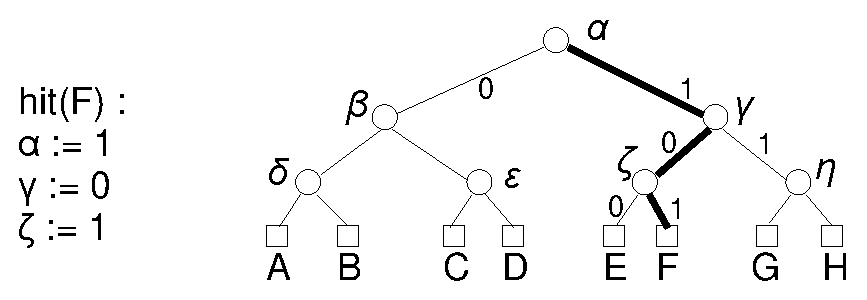
\includegraphics[width=0.7\textwidth]{2.theor/plruhit}\\
  \caption{Попадание для стратегия вытеснения \PseudoLRU
  (16-ассоциативная таблица)}\label{pseudo_lru_hit}
\end{figure}

На основании пометок вершин определяется и лист, по которому надо произвести
вытеснение.
%Вытесняющий тег помещается в дереве на место вытесняемого.
Из корня дерева строится <<вытесняющий путь>> (он будет единственным),
вытесняться будут данные листа этого пути. В <<вытесняющем пути>> нужная
исходящая дуга каждой очередной вершины должна иметь пометку, противоположную
пометке этой вершины. Т.е. если вершина помечена цифрой 0, значит дуга пути из
этой вершины идет вправо, если вершина помечена цифрой 1 -- влево. Затем пометки
вершин дерева изменяются так, как будто происходит попадание на <<вытесняемый>>
лист. Пример того, как определяется вытесняемый элемент, показан на
рис.~\ref{pseudo_lru_miss}. Цветом показаны пометки нелистовых вершин: черным
вершинам соответствует пометка 1, белым
-- 0. В изображенном на рисунке дереве в качестве вытесняемого листа будет
выбран D, к которому ведет путь $\alpha-\beta-\varepsilon$.

\begin{figure}[h] \center
  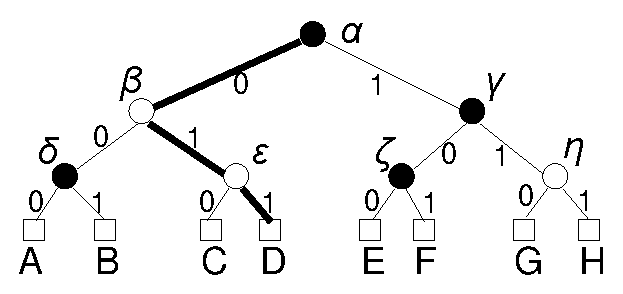
\includegraphics[width=0.5\textwidth]{2.theor/plrumiss}\\
  \caption{Определение вытесняемого элемента для стратегия вытеснения
  \PseudoLRU (16-ассоциативная таблица)}\label{pseudo_lru_miss}
\end{figure}


\subsubsection{Каноническое определение \PseudoLRU на битовой строке}

Для каждого региона хранится битовая строка $\beta$ длины $w-1$, где $w$ --
ассоциативность таблицы. Стратегия вытеснения определяется как процесс изменения
бит этой битовой строки.

Во многих книгах приводятся следующее определение стратегии
вытеснения \PseudoLRU для случая
$w=4$~\cite{FundamentalOfComputerOrganizationAndDesign} (в этом
случае для каждого региона выделяется 3 бита $B_1$, $B_2$ и $B_3$):
$$ \left[
  \begin{array}{c|ccc}
          & B_1 & B_2 & B_3 \\ \hline
    \pi_0 & 0 & 0 & \textsf{X} \\
    \pi_1 & 0 & 1 & \textsf{X} \\
    \pi_2 & 1 & \textsf{X} & 0 \\
    \pi_3 & 1 & \textsf{X} & 1 \\
  \end{array}
\right]
$$

Строки в регионе пронумерованы числами от 0 до $w-1$. При попадании на строку
региона с номером $i$ задействована строка матрицы, начинающаяся с $\pi_i$. Биты
$\beta$, напротив которых в строке матрицы находится \textsf{X}, не меняются.
Биты $\beta$, напротив которых в $i$'й строке находится число, принимают
значение, равное этому числу.

При промахе надо определить номер вытесняемой строки. Для этого используется
инвертированная форма той же матрицы:
$$
\left[
  \begin{array}{ccc|c}
    B_1 & B_2 & B_3 & \\ \hline
    1 & 1 & \textsf{X} & \rightarrow \pi_0 \\
    1 & 0 & \textsf{X} & \rightarrow \pi_1 \\
    0 & \textsf{X} & 1 & \rightarrow \pi_2 \\
    0 & \textsf{X} & 0 & \rightarrow \pi_3 \\
  \end{array}
\right]
$$

Выбирается строка, соответствующая текущему состоянию бит $B_1$,
$B_2$ и $B_3$: если напротив бита в строке находится число, бит
должен быть равен этому числу -- если напротив бита в строке
находится \textsf{X}, то требования на соответствующий бит нет.
Подходящая строка всегда будет существовать и она будет
единственной.

Изменение $\beta$ обычно демонстрируют на бинарном дереве. $\beta$ составляется из пометок вершин дерева, начиная с корня и далее по слоям от левых к правым вершинам (см.
рис.~\ref{plru_bittree}).

\begin{figure}[h] \center
  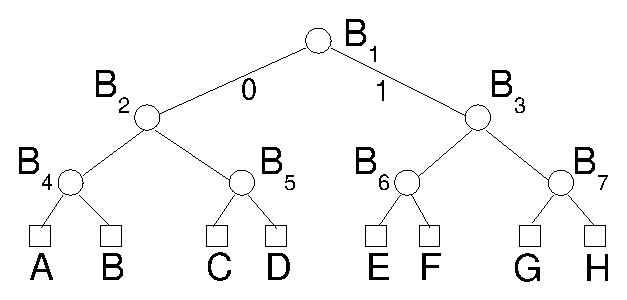
\includegraphics[width=0.5\textwidth]{1.review/plru}\\
  \caption{Битовая строка в бинарном дереве}\label{plru_bittree}
\end{figure}

Формализованное описание для всех допустимых $w$ в литературе не
приводится. Однако в дальнейшем для формулирования и доказательства
утверждений про стратегию вытеснения \PseudoLRU такое описание будет
необходимо. Для $w=8$ стратегия будет задаваться следующей матрицей:
$$
\left[
  \begin{array}{c|ccccccc}
          & B_1 & B_2 & B_3 & B_4 & B_5 & B_6 & B_7 \\ \hline
    \pi_0 & 0 & 0 & \textsf{X} & 0 & \textsf{X} & \textsf{X} & \textsf{X} \\
    \pi_1 & 0 & 0 & \textsf{X} & 1 & \textsf{X} & \textsf{X} & \textsf{X} \\
    \pi_2 & 0 & 1 & \textsf{X} & \textsf{X} & 0 & \textsf{X} & \textsf{X} \\
    \pi_3 & 0 & 1 & \textsf{X} & \textsf{X} & 1 & \textsf{X} & \textsf{X} \\
    \pi_4 & 1 & \textsf{X} & 0 & \textsf{X} & \textsf{X} & 0 & \textsf{X} \\
    \pi_5 & 1 & \textsf{X} & 0 & \textsf{X} & \textsf{X} & 1 & \textsf{X} \\
    \pi_6 & 1 & \textsf{X} & 1 & \textsf{X} & \textsf{X} & \textsf{X} & 0 \\
    \pi_7 & 1 & \textsf{X} & 1 & \textsf{X} & \textsf{X} & \textsf{X} & 1 \\
  \end{array}
\right]
$$

Следующее утверждение~\ref{wMinus1PseudoLRU} дает алгоритм
преобразования списка бит\\ $B_1, B_2, ..., B_{w{-}1}$ в результате
обращения в таблицу. В его формулировке применяется двоичное
разложение. Биты разложения обозначаются последовательностью от
старших бит к младшим (т.е. список ($x_1~x_2~\dots~x_n$) обозначает
число $x_n + 2\cdot x_{n-1} + 4\cdot x_{n-2} + \dots + 2^n\cdot x_1$, $x_i \in
\{0,
1\}$ для $i = 1, 2, \dots, n$). Например, 1 = (0 0 1), 6 = (1 1 0).

Везде далее символ $W$ будет обозначать $\log_2 w$. По определению
стратегии вытеснения \PseudoLRU $W$ будет натуральным числом.

\begin{utv}[$(w{-}1)$-представление стратегии вытеснения
\PseudoLRU]\label{wMinus1PseudoLRU}При попадании строки с позицией
$i = (i_1~i_2~\dots~i_W)$ происходит следующее изменение бит $B_1,
B_2, ..., B_{w{-}1}$:

\parbox{0.3\textwidth}{
  $$ \begin{array}{l}
  B_{k_1} := i_1 \\
  B_{k_2} := i_2 \\
  B_{k_3} := i_3 \\
  ...\\
  B_{k_W} := i_W \\
  \end{array}$$
} \vline
\parbox{0.7\textwidth}{
  $$ \begin{array}{l}
  k_1 = (1) \\
  k_2 = (1~i_1) \\
  k_3 = (1~i_1~i_2) \\
  ...\\
  k_W = (1~i_1~i_2~\dots~i_{W{-}1}) \\
  \end{array} $$
}
\\[1cm]

При промахе позиция вытеснения $i = (i_1~i_2~\dots~i_W)$ определяется
следующим образом:

\parbox{0.3\textwidth}{
  $$ \begin{array}{l}
  i_1 = \neg B_{k_1} \\
  i_2 = \neg B_{k_2} \\
  i_3 = \neg B_{k_3} \\
  ...\\
  i_W = \neg B_{k_W} \\
  \end{array}$$
} \vline
\parbox{0.7\textwidth}{
  $$ \begin{array}{l}
  k_1 = (1) \\
  k_2 = (1~\neg B_{k_1}) \\
  k_3 = (1~\neg B_{k_1}~\neg B_{k_2}) \\
  ...\\
  k_W = (1~\neg B_{k_1}~\neg B_{k_2}\dots\neg B_{k_{W{-}1}}) \\
  \end{array} $$
}
\\[0.5cm]

Кроме того при кэш-промахе после определения позиции $i$ делается
преобразование бит $B_1, B_2, ..., B_{w{-}1}$ так, как в случае
попадания на $\pi_i$.
\end{utv}

Нехитрые расчеты показывают, что это утверждение верно для $w$ = 4 и 8.

\subsubsection{Определение \PseudoLRU на ветвях бинарного
дерева}\label{sec:PseudoLRUonBranches}

Здесь будет показано, как из канонического определения \PseudoLRU
получить формулировку \PseudoLRU с точки зрения одной строки региона~\cite{my_lomonosov_2010}
(каноническое определение рассматривает весь регион целиком и
для него формулирует правила работы с последовательностью бит $B_1,
B_2, ..., B_{w{-}1}$). Это определение ранее не встречалось в
литературе.

Сначала этот переход покажем на примере $w=4$. Первый шаг --- это
смена <<состояния>>: вместо последовательности бит $B_1, B_2, ...,
B_{w-1}$ будем рассматривать последовательность векторов бит
$\beta_0, \beta_1, \dots, \beta_{w-1}$ размера $W$. Каждый $\beta_i$
соответствует $i$'й листовой вершине бинарного дерева. Попадание
меняет теперь атрибуты не внутренних вершин дерева, а листовых.
Каждый $\beta_i$ будет представляться списком длины $W$ -- путь от
корня дерева к $i$'й листовой вершине: $\beta_0$ соответствует
($B_1$ $B_2$), $\beta_1$ соответствует ($B_1$ $\neg B_2$), $\beta_2$
соответствует ($\neg B_1$ $B_3$) и $\beta_3$ соответствует ($\neg
B_1$ $ \neg B_3$).\\[0.5cm]

\parbox{0.2\textwidth}{ \centering
  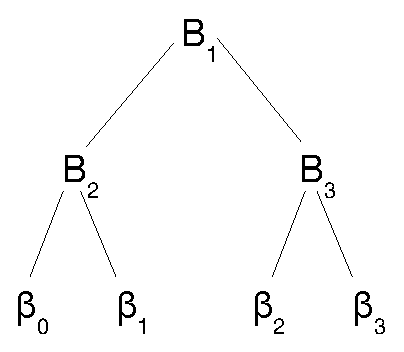
\includegraphics[width=0.2\textwidth]{1.review/btree}
}
\parbox{0.25\textwidth}{
$$ \left[
  \begin{array}{c|ccc}
          & B_1 & B_2 & B_3 \\ \hline
    \pi_0 & 0 & 0 & \textsf{X} \\
    \pi_1 & 0 & 1 & \textsf{X} \\
    \pi_2 & 1 & \textsf{X} & 0 \\
    \pi_3 & 1 & \textsf{X} & 1 \\
  \end{array}
\right]
$$
} $\stackrel{1}{\longrightarrow}$ %\vline
\parbox{0.4\textwidth}{
$$ \left[
  \begin{array}{c|cccc}
          & \beta_0 & \beta_1 & \beta_2 & \beta_3 \\ \hline
    \pi_0 & (0~0) & (0~1) & (1~\textsf{X}) & (1~\textsf{X}) \\
    \pi_1 & (0~1) & (0~0) & (1~\textsf{X}) & (1~\textsf{X}) \\
    \pi_2 & (1~\textsf{X}) & (1~\textsf{X}) & (0~0) & (0~1) \\
    \pi_3 & (1~\textsf{X}) & (1~\textsf{X}) & (0~1) & (0~0) \\
  \end{array}
\right]
$$
}

Заметим, что получилась симметричная матрица. На пересечении $\pi_i$
и $\beta_j$ располагается вектор, задающий изменение вектора в $j$'й
листовой вершине дерева при попадании $i$'й листовой вершины
дерева. Назовем позицию $i \oplus j$ \emph{относительной позицией}
$i$ относительно $j$. Рассмотрим отдельно каждый столбец
получившейся матрицы и переставим элементы столбца в порядке
увеличения относительных позиций.

\parbox{0.2\textwidth}{
$$ \left[
  \begin{array}{c|c}
          & \beta_0 \\ \hline
    \pi_0 & (0~0) \\
    \pi_1 & (0~1) \\
    \pi_2 & (1~\textsf{X}) \\
    \pi_3 & (1~\textsf{X}) \\
  \end{array}
\right]
$$
}\parbox{0.2\textwidth}{
$$ \left[
  \begin{array}{c|c}
          & \beta_1 \\ \hline
    \pi_0 & (0~1) \\
    \pi_1 & (0~0) \\
    \pi_2 & (1~\textsf{X}) \\
    \pi_3 & (1~\textsf{X}) \\
  \end{array}
\right]
$$
}\parbox{0.2\textwidth}{
$$ \left[
  \begin{array}{c|c}
          & \beta_2 \\ \hline
    \pi_0 & (1~\textsf{X}) \\
    \pi_1 & (1~\textsf{X}) \\
    \pi_2 & (0~0) \\
    \pi_3 & (0~1) \\
  \end{array}
\right]
$$
}\parbox{0.2\textwidth}{
$$ \left[
  \begin{array}{c|c}
          & \beta_3 \\ \hline
    \pi_0 & (1~\textsf{X}) \\
    \pi_1 & (1~\textsf{X}) \\
    \pi_2 & (0~1) \\
    \pi_3 & (0~0) \\
  \end{array}
\right]
$$
} $\stackrel{2}{\stackrel{\longrightarrow}{\pi^i_j \equiv \pi_{i
\oplus j}}}$

\parbox{0.24\textwidth}{
$$ \left[
  \begin{array}{c|c}
          & \beta_0 \\ \hline
    \pi^0_0 \equiv \pi_0 & (0~0) \\
    \pi^0_1 \equiv \pi_1 & (0~1) \\
    \pi^0_2 \equiv \pi_2 & (1~\textsf{X}) \\
    \pi^0_3 \equiv \pi_3 & (1~\textsf{X}) \\
  \end{array}
\right]
$$
}\parbox{0.24\textwidth}{
$$ \left[
  \begin{array}{c|c}
          & \beta_1 \\ \hline
    \pi^1_0 \equiv \pi_1 & (0~0) \\
    \pi^1_1 \equiv \pi_0 & (0~1) \\
    \pi^1_2 \equiv \pi_3 & (1~\textsf{X}) \\
    \pi^1_3 \equiv \pi_2 & (1~\textsf{X}) \\
  \end{array}
\right]
$$
}\parbox{0.24\textwidth}{
$$ \left[
  \begin{array}{c|c}
          & \beta_2 \\ \hline
    \pi^2_0 \equiv \pi_2 & (0~0) \\
    \pi^2_1 \equiv \pi_3 & (0~1) \\
    \pi^2_2 \equiv \pi_0 & (1~\textsf{X}) \\
    \pi^2_3 \equiv \pi_1 & (1~\textsf{X}) \\
  \end{array}
\right]
$$
}\parbox{0.24\textwidth}{
$$ \left[
  \begin{array}{c|c}
          & \beta_3 \\ \hline
    \pi^3_0 \equiv \pi_3 & (0~0) \\
    \pi^3_1 \equiv \pi_2 & (0~1) \\
    \pi^3_2 \equiv \pi_1 & (1~\textsf{X}) \\
    \pi^3_3 \equiv \pi_0 & (1~\textsf{X}) \\
  \end{array}
\right]
$$
}

После перехода к относительным позициям ($\pi^i_j$ -- это позиция
$\pi_j$ относительно $\pi_i$) все столбцы получились одинаковыми.
Иными словами, \emph{алгоритм изменения региона согласно стратегии
вытеснения \PseudoLRU на относительных позициях инвариантен
относительно абсолютной позиции вытесняемой строки}. Строка вытесняется в
том случае, когда её вектор равен (1 1). Следующая теорема
формально доказывает этот факт.

Будем называть \emph{\PseudoLRU-ветвью позиции $i$} вектор
$(B_{k_1}^{\sigma_1}~B_{k_2}^{\sigma_2}~\dots~B_{k_W}^{\sigma_W})$,
в котором $\sigma_j = \neg i_j$, $k_j = (1~i_1~i_2~\dots~i_{j-1})$,
$j = 1, 2, \dots, W$, $i = (i_1~i_2~\dots~i_W)$ (двоичное
разложение). Степени определены стандартным образом: $B^1 \equiv B,
B^0 \equiv \neg B$.

\begin{theorem}[Инвариантность преобразования \PseudoLRU-ветвей относительными
позициями]\label{thm_pseudoLRU_invariant} \PseudoLRUInvariant
\end{theorem}
Доказательство теоремы приведено в приложении~\ref{sec:proofs}.

Доказанный факт позволяет сформулировать определение стратегии
вытеснения \PseudoLRU, сфокусированное не на изменении атрибутов строк всего
региона,
а на изменении атрибутов одной строки. На этом определении
будут базироваться применения предлагаемых методов генерации
ограничений для стратегии вытеснения \PseudoLRU.

\begin{utv}[формулировка \PseudoLRU на ветвях бинарного дерева]
Сопоставим строке вектор длины $W$. Каждая инструкция, обращающаяся к этой
строке,
делает её вектор равным (0 0 ... 0). Строка является вытесняемой в
том и только в том случае, если её вектор равен (1 1 ... 1).
Влияние других инструкций определяется относительной позицией их
строки относительно позиции данной строки. Если относительная позиция
принадлежит области $[\frac{w}{2^k},~\frac{w}{2^{k-1}}), k =
1,2,...,W$, то первые $k{-}1$ элементов вектора становятся равными
0, $k$'й элемент вектора становится равным 1, остальные элементы
вектора не меняются.
\end{utv}

Вектор длины $W$ будет соответствовать пути из корня бинарного
дерева в листовую вершину, соответствующую данной строке.
Будем называть процесс изменения элемента вектора
\emph{перекрашиванием вершины ветви}. Элементы вектора, равные 0,
будем называть \emph{белыми}, элементы вектора, равные 1, будем
называть \emph{черными}.

Говоря в терминах бинарного дерева, нелистовая вершина в ветви к
данной листовой вершине будет <<белой>>, если дуга пути от нее идет
налево и она помечена цифрой 1 или дуга пути от нее идет направо и она
помечена цифрой 0 (т.е. в том случае, когда направление дуги из нее
соответствует пометке этой дуги). Нелистовая вершина будет
называться <<черной>>, если направление дуги пути из нее не соответствует
пометке этой дуги. Вытесняется та строка, путь к которой
полностью состоит из несоответствующих дуг. На рисунке~\ref{recolor}
изображен процесс перекрашивания ветви, ведущей в А, под действием
попадания в C (для сокращения показана только ветвь в А без
остальной части дерева). Так как путь из корня в C совпадает из
верхних двух вершин, то они перекрашиваются в белый цвет. Дуга из
третьей вершины пути в С не совпадает с дугой пути в А, поэтому
третья вершина перекрашивается в черный цвет. Остальные вершины
ветви остаются без изменений.

\begin{figure}[h] \center
  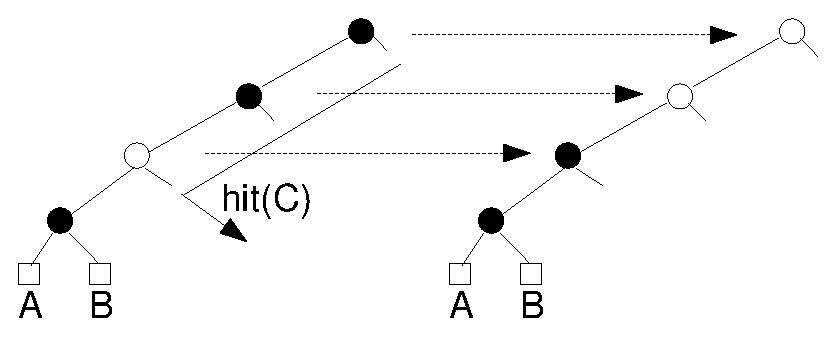
\includegraphics[width=0.8\textwidth]{1.review/recolor}\\
  \caption{Перекрашивание ветви в А}\label{recolor}
\end{figure}


Определение стратегии вытеснения \PseudoLRU на ветвях дерева
является связующим звеном между каноническим определением (например,
на битовой строке) и определением с помощью таблицы вытеснения,
поскольку ветвь -- это и есть позиция, которая меняется точно так
же, как и позиция в перестановке согласно таблице вытеснения.


%%%%%%%%%%%%%%%%%%%%%%%%%%%%%%%%%%%%%%%%%%%%%%%%%%%%%%%%%%%%%%%%%%%%

\section{Метод функций полезности записи стратегии вытеснения в виде ограничений}\label{sec:usefulness_functions}

%{\footnotesize В разделе рассматривается метод составления ограничений для
%описания стратегии вытеснения, для которой удается определить функционал
%вытеснения. Стратегия вытеснения описывается ограничением сверху на количество \emph{полезных} инструкций (т.е. помогающих вытеснению).
%В разделе приведены определения полезных инструкций и способы составления ограничений для трех
%наиболее часто используемых в микропроцессорах стратегий вытеснения -- \LRU, \FIFO и \PseudoLRU. Освещается понятие \emph{монотонного функционала вытеснения}, который является залогом более
%простой системы ограничений.}

В данном разделе процесс вытеснения будет представляться как изменение значений
системы функций, отображающих ключи в целые числа. Каждая инструкция изменяет значения функций по
всем ключам. Пример процесса изменения значения функции для некоторого ключа изображен на рисунке~\ref{fig:graphic}.

\begin{figure}[h] \center
  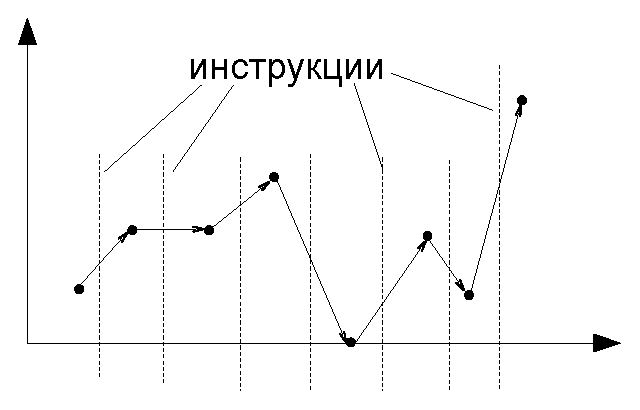
\includegraphics[width=0.5\textwidth]{2.theor/graphic}\\
  \caption{К определению стратегии вытеснения}\label{fig:graphic}
\end{figure}

Говоря формально, пусть $\alpha, \beta, \dots, \gamma$ --- одноместные функции,
отображающие ключи в целые числа. Для каждой инструкции определены функции
изменения значений функций $\alpha, \beta, \dots, \gamma$:
$$\parbox{2.5cm}{in-parallel\\forall x~}\left|\begin{array}{l}
\alpha(x) := A_I(k, \alpha, \beta, \dots, \gamma)\\
\beta(x) := B_I(k, \alpha, \beta, \dots, \gamma)\\
\dots\\
\gamma(x) := C_I(k, \alpha, \beta, \dots, \gamma)\\
\end{array}\right.
$$

Обновления $\alpha, \beta, \dots, \gamma$ выполняются одновременно. $I$ ---
инструкция, $k$ --- ключ в этой инструкции. Функции $A_I$, $B_I$, \dots, $C_I$
отражают влияние обращения по некоторому ключу на другой произвольный ключ.
Возможны следующие случаи (в качестве $x$ рассматривается произвольный ключ, не
обязательно <<находящийся>> в регионе):
\begin{itemize}
    \item в результате обращения по ключу $k$ ключ $x$ <<попадает>> в регион
(т.е. в регион добавляется строка с ключом $x$);
    \item в результате обращения по ключу $k$ ключ $x$ <<вытесняется>> из
региона (т.е. из региона удаляется строка с ключом $x$);
    \item в результате обращения по ключу $k$ состояние ключа $x$ в регионе не
меняется.
\end{itemize}

Этим ситуациям как раз и ставятся в соответствие классы значений функций
$\alpha, \beta, \dots, \gamma$, а функции $A_I$, $B_I$, \dots, $C_I$
осуществляют переход между этими классами. Тем самым стратегия вытеснения будет
описана в виде изменения таких <<счетчиков>> $\alpha, \beta, \dots, \gamma$.

Формально это правило выражается следующим образом. Будем называть функцию
$\alpha$ \emph{функционалом вытеснения} для заданной стратегии вытеснения, если
одновременно выполнены следующие свойства:
\begin{enumerate}
  \item существуют константы $\alpha_{min}$ и $\alpha_{max}$ такие, что
$\alpha_{min} \leqslant \alpha_{max}$;
  \item для любого ключа $x$ $\alpha_{min} \leqslant \alpha(x) \leqslant
\alpha_{max}$ тогда и только тогда, когда $x$ находится в регионе по определению
стратегии вытеснения;
  \item для любого ключа $k$ $A_I(k, \alpha,\beta,\dots,\gamma) (k) =
\alpha_{min}$;
  \item $\exists! \phi: \mbox{~ключ~}^2 \times \mathds{Z}^{2\cdot n} \rightarrow
\mathds{Z}$, где $n$ --- количество функций во множестве
$\{\alpha,\beta,\dots,\gamma\}$, такая, что для любого ключа $x$ $$A_I(k,
\alpha,\beta,\dots,\gamma)(x) \equiv \phi(k, \alpha(k), \beta(k), \dots,
\gamma(k), x, \alpha(x), \beta(x), \dots, \gamma(x))$$ иными словами, в функции
изменения функционала вытеснения разрешается обращаться только к $k$ и тому ключу,
для которого определяется функционал вытеснения;
  \item $\exists! x^* : \alpha(x^*) = \alpha_{max}$;
  \item перед любым неуспешным обращением (промахом) $\alpha(x^*) =
\alpha_{max}$ тогда и только тогда, когда $x^*$ есть <<вытесняемый>> ключ по
определению стратегии вытеснения (т.е. строка с ключом $x^*$ является
вытесняемой при данном обращении по определению стратегии вытеснения);
\end{enumerate}

Пример функционала вытеснения: $\alpha$ --- счетчик количества обращений к строке
для стратегии вытеснения \LRU. Обращение по тому же счетчику делает $\alpha$
равным 1, по другому ключу --- увеличивает $\alpha$ на единицу. Вытесняемым
считается ключ, чей счетчик равен $w$ --- количеству строк в регионе. Проверим
определение функционала вытеснения:
\begin{enumerate}
    \item $\alpha_{min}$ = 1, $\alpha_{max}$ = $w$, $1 \leqslant w$;
    \item верно, что счетчик больше $w$ тогда и только тогда, когда $x$ не
находится в регионе; в противном случае, было бы возможно успешное обращение к
большему числу строк, чем хранится в регионе;
    \item по условию обращение по тому же счетчику делает $\alpha$ равным 1, что
и есть $A_I(x;...)(x) = 1$;
    \item изменение одного счетчика независимо от изменений других счетчиков;
    \item такой $x^*$ существует, ибо в противном случае было бы возможно
успешное обращение к большему числу строк, чем хранится в регионе; такой $x^*$
единственный, поскольку каждая инструкция меняет каждый счетчик и в минимальное
значение $\alpha$ изменяется лишь по единственному ключу.
\end{enumerate}

Пусть для стратегии вытеснения сформулирован функционал вытеснения. Будем называть
инструкцию (обращение по некоторому ключу) \emph{полезной для вытеснения} ключа
$x$ (или просто, \emph{полезной}), если она увеличивает функционал вытеснения по
ключу $x$ на этапе его монотонного увеличения до максимального значения (см.
рис.~\ref{useful}).

\begin{figure}[h] \center
  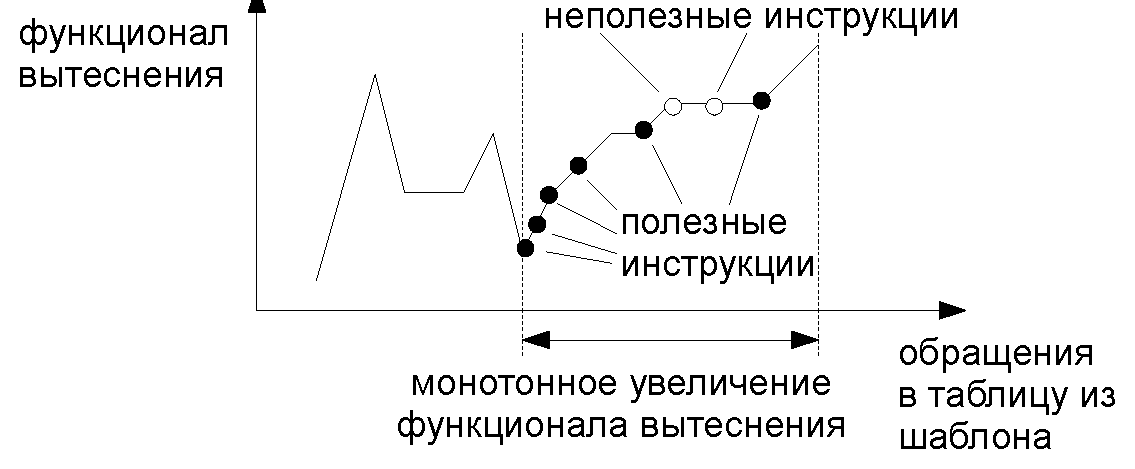
\includegraphics[width=0.6\textwidth]{2.theor/useful}\\
  \caption{К определению полезных инструкций}\label{useful}
\end{figure}

Тогда вытеснение будет происходить в том случае, когда количество
полезных инструкций превысит некоторое константное количество.
И вытеснение не будет происходить, если количество полезных инструкций
не превысит некоторой константной верхней границы.

\emph{Функцией полезности} инструкции будем называть характеристическую\\ функцию
свойства инструкции быть полезной. Т.е. функция полезности для полезной
инструкции равна 1, для остальных инструкций равна 0. В дальнейших формулировках
функцией полезности могут обозначаться просто предикаты, что надо воспринимать
как функцию, равную 1 при истинном предикате и 0 при ложном.

Тем самым ограничение (constraint) <<быть вытесненным>> представимо в виде
ограничения сверху на сумму функций полезности инструкций, составляющих тестовый
шаблон: $\sum_{i=1}^n u_x(k_i) < N$, где $u_x(k_i)$ -- функция полезности
обращения по ключу $k_i$ для ключа $x$. Если будет важен регион, в который
происходит обращение, то он также будет указываться: $u_{x,r}(k_i, r_i)$. Еще
раз подчеркну, что представленное неравенство выражает ограничение количества
полезных инструкций, каждая полезная инструкция увеличивает функционал вытеснения,
значит при должном количестве полезных инструкций функционал вытеснения примет
<<максимальное>> значение ($\alpha_{max}$) и произойдет вытеснение.

Функции полезности, как и функционалы вытеснения, не являются единственными.
Например, для стратегии вытеснения \LRU возможны следующие две различные функции
полезности (далее для одной из них будет формально показано, что она
действительно является функцией полезности) (функции вытеснения приведены для
случая полностью ассоциативной таблицы):
\begin{itemize}
  \item $u_x(x_i) \equiv (x \notin \{x_i, x_{i+1}, ..., x_n\} \wedge
\bigwedge\limits_{j=1,2,...,i-1} (x \in \{x_j, x_{j+1}, ..., x_{i-1}\} \vee x_j
\neq x_i))$ -- инструкция считается полезной, если она расположена после
последнего обращения к $x$ и с того момента является первым обращением к своему
ключу; нетрудно заметить, что это в чистом виде определение \LRU, изображенное на рисунке~\ref{fig:lru1}: обращение по ключу $x_j$, который расположен после ключа $x$, передвигает $x$ к концу вектора, за концом происходит вытеснение; первые обращения по ключам после последнего обращения к $x$ -- это и есть именно те обращения, где $x$ сдвигается
к концу; иначе говоря, полезная инструкция сдвигает $x$ к концу, приближая его к
вытеснению;
  \item $u_x(x_i) \equiv (x \notin \{x_i, x_{i+1}, ..., x_n\} \wedge x_i \notin
\{x_{i+1}, x_{i+2}, ..., x_n\})$ -- инструкция считается полезной, если она
расположена после последнего обращения к $x$ и является последним обращением к
своему ключу перед финальным обращением к $x$; т.е. в таблице хранятся некоторые
ключи, есть некоторый ключ $x$, есть последовательность других обращений (их
ключи есть $x_i$, ..., $x_n$), полезными будут лишь последние к ним обращения
(среди $x_i$, ..., $x_n$ могут быть равные), т.е. все полезные инструкции вместе
образуют (по разу) все различные ключи.
\end{itemize}

Тем самым, метод функций полезности состоит в следующем:
\begin{enumerate}
  \item выделить функционал вытеснения $\alpha$;
  \item выделить определение полезной инструкции;
  \item записать функцию полезности $u_{x,r}(x_i, r_i)$ для инструкции с ключом
$x$ и регионом $r$;
  \item определить $\alpha_{max}$;
  \item составить ограничение для свойства <<$x$ вытеснен>> в виде
$\sum\limits_{i=1}^n u_{x,r}(x_i, r_i) > \alpha_{max}$ и для свойства <<$x$ не
вытеснен>> в виде $\sum\limits_{i=1}^n u_{x,r}(x_i,r_i) \leqslant \alpha_{max}$.
\end{enumerate}

Ключевой вопрос при применении метода функций полезности --- это, конечно, выбор
функционала вытеснения. От него в том числе будет зависеть сложность функции
полезности и генерируемых ограничений.

В некоторых случаях функционал вытеснения может быть получен из таблицы вытеснения
(policy table). А именно, если вытеснение происходит с позиции с максимальным
номером (т.е. в последней строке отсутствует число $w{-}1$), а в результате
попадания ключ переносится в самое начало (т.е. второй столбец имеет вид (0 1 2
... $w{-}1$ $m$)$^T$ ). Тогда $\alpha$ --- это позиция ключа в перестановке,
$\alpha_{min}$ = 0, $\alpha_{max} = w{-}1$. Этими свойствами, например, обладают
таблицы вытеснения \LRU (см.рис.~\ref{fig:PolicyTableLRU8}) и
\PseudoLRU~\cite{policy_tables}.

В отличие от метода диапазонов вытеснения при использовании функций полезности
не происходит выделение участка тестового шаблона, непосредственно влияющего на
вытеснение. Считается, что это влияние начинается с момента появления строки в
таблице. Другое дело, что одни инструкции влияют на ее вытеснение (это и есть
<<полезные>> инструкции), а другие -- нет.


\subsection{Метод функций полезности для стратегии вытеснения \LRU}

\LRU (Least Recently Used) --- это стратегия вытеснения,
определяющая вытесняемые данные как наименее используемые. Она
эффективна для алгоритмов, обладающих свойством локальности данных,
т.е. чаще использующих те данные, к которым недавно происходило
обращение. Эта стратегия используется, например, в микропроцессорах
архитектуры MIPS~\cite{mips64II}.

Стратегия вытеснения \LRU обычно определяется с использованием
счетчиков обращений. Для каждой строки таблицы
вводится счетчик обращений к ней. Каждое обращение увеличивает
счетчик. Вытесняемым в регионе будет элемент с минимальным счетчиком его строк.
%Поскольку границы значений счетчика неизвестны, формулирование
%функционала вытеснения на основе счетчика провести сложно.

Другой способ описания \LRU основан на введении порядка на строках региона (т.е.
регион представляется вектором строк). После каждой инструкции элементы этого вектора переупорядочиваются, \emph{переставляются}, согласно следующим правилам (см.рис.~\ref{fig:lru1}):
\begin{itemize}
\item при попадании элемент, соответствующий адресу инструкции,
перемещается в начало, остальные элементы от первого до данного
сдвигаются на одну позицию;
\item при промахе вытесняется последний элемент, в начало
вставляется элемент, вызвавший промах.
\end{itemize}

\begin{figure}[h] \center
  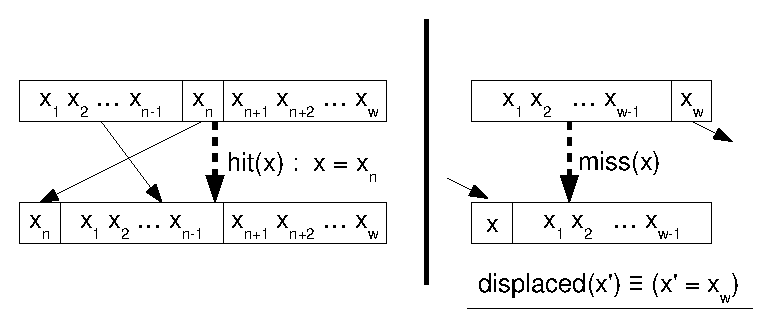
\includegraphics[width=0.6\textwidth]{2.theor/lru1}\\
  \caption{Стратегия вытеснения \LRU (w --- ассоциативность) на
перестановках}\label{fig:lru1}
\end{figure}

Позиция ключа, индекс, в таком векторе ограничена, единственна, ее изменение допускает представление, независимое от других ключей. Тем самым \emph{<<позиция>> ключа может быть функционалом вытеснения}.

Функция изменения этого функционала выглядит следующим образом:\\

\parbox{0.5\textwidth}{ \tt
$A_{\mbox{hit}}(k, \alpha)(x) \equiv$\\
if $\alpha(x) > w$ then $\alpha(x)$\\
elsif $\alpha(k) > \alpha(x)$ then $\alpha(x)+1$\\
elsif $\alpha(k) = \alpha(x)$ then $1$\\
else $\alpha(x)$ endif%
}\parbox{0.5\textwidth}{\tt
$A_{\mbox{miss}}(k, \alpha)(x) \equiv$\\
if $k = x$ then $1$\\
elsif $\alpha(x) > w$ then $\alpha(x)$\\
else $\alpha(x) + 1$ endif}\\

Согласно методу полезной будет считаться инструкция, увеличивающая позицию, т.е.
переставляющая соответствующий ключ к концу. Такими инструкциями являются все
промахи (поскольку они
вытесняют последний элемент вектора с передвижением всех остальных на одну
позицию к концу, т.е. будет передвинут и данный рассматриваемый элемент) и
попадания к элементам, находившимся ближе к концу, чем данный вытесняемый
(потому как при попадании они
передвинутся в самое начало, а все элементы от начала и до них сдвинутся на одну
позицию к концу, в том числе и рассматриваемый).

Осталось выразить эту идею в виде ограничений~\cite{my_ewdts_2009}.
Учет полезных инструкций начинается уже в инициализирующей последовательности,
тем самым необходимо будет сформулировать функции полезности и для
инициализирующих инструкций.

Следующая теорема описывает функцию полезности для \LRU ($m$ --- количество
инициализирующих инструкций):

\begin{theorem}[Выражение свойства <<быть вытесненным>> для \LRU]\label{correct_mirror_LRU} \LRUusefuls
\end{theorem}

\begin{proof}
По определению стратегии вытеснения \LRU <<$k$ не вытеснен из региона $R$ согласно определению на перестановках>> эквивалентно тому, что после последнего обращения к $k$ в $R$ происходит не более $w$ обращений по различным ключам в регион $R$. Несложно убедиться, что это количество выражается следующей формулой: $$|\{s_i| R = R(s_i) \wedge s \notin \{s_i, ..., s_{m+n}\}\}|$$
Однако это же число можно записать другим образом, чтобы исключить повторения одинаковых $s_i$:
$$|\{s_i| R = R(s_i) \wedge s \notin \{s_i, ..., s_{m+n}\} \wedge s_i \notin \{s_{i+1}, ..., s_{m+n}\}\}|$$

Ввиду конечности последовательности $\langle s_i, ..., s_{m+n}\rangle$ в нем всегда найдется последнее вхождение $s_i$ --- множество последних вхождений всех элементов списка равно множеству всех элементов списка.

Представленная мощность множества и есть требуемая сумма.
\end{proof}

Из теоремы~\ref{correct_mirror_LRU} следует система уравнений для
описания обращений по ключу $k$ в регион $R$ согласно методу функций полезности
для \LRU: \begin{itemize}
\item $k$ еще не вытеснен из региона $R$:
$$
\left\{\begin{array}{l} (k||R) \in \{(t_1||r_1), ..., (t_m||r_m), (k_1||R_1),
..., (k_n||R_n)\}\\
\sum\limits_{i=1}^m u_{k,R}(t_i||r_i) + \sum\limits_{i=1}^n u_{k,R}(k_i||R_i) <
w\\
\{(t_1||r_1), ..., (t_m||r_m)\} - \mbox{все разные}\\
\end{array} \right.
$$
\item $k$ вытеснен из региона $R$:
$$
\left\{\begin{array}{l} (k||R) \in \{(t_1||r_1), ..., (t_m||r_m), (k_1||R_1),
..., (k_n||R_n)\}\\
\sum\limits_{i=1}^m u_{k,R}(t_i||r_i) + \sum\limits_{i=1}^n u_{k,R}(k_i||R_i)
\geqslant w\\
\{(t_1||r_1), ..., (t_m||r_m)\} - \mbox{все разные}\\
\end{array} \right.
$$
\end{itemize}


%Для этого удобно использовать утверждение~\ref{hit_miss_human}. Символом
%$\lambda_\delta$ будет обозначаться элемент начального
%состояния таблицы с индексом $\delta$ по порядку \LRU, $1 \leqslant \delta \leqslant w$. Индекс 1 обозначает самый молодой элемент, индекс $w$ обозначает самый старый элемент.
%
%Применение полезностей эффективно в том случае, когда домен имеет
%небольшой размер. В этом случае можно перебрать все элементы
%домена (это и будут $\lambda_\delta$) и составить для них свои
%полезности, причем для каждого элемента будет известен индекс по
%порядку \LRU ($\delta$). Ограничение, описывающее стратегию
%вытеснения, будет при этом иметь вид дизъюнкции по элементам домена.
%
%Если вытесняемый элемент был в начальном состоянии (пусть это
%$\lambda_\delta$) и к нему не было обращений, то для его вытеснения
%необходимо $w-\delta + 1$ полезных инструкций, потому что столько
%раз надо подвинуть элемент с индексом $\delta$ в \LRU-списке в
%сторону к концу (к элементам с индексом $w$), чтобы он вышел за
%границу списка (иными словами, чтобы он был вытеснен).
%
%Если вытесняемый элемент был в начальном состоянии и к нему было
%обращение, то для его вытеснения необходимо $w$ инструкций, так как
%во время обращения элемент был поставлен в самое начало \LRU-списка.
%То же справедливо для внесенных в кэширующий буфер новых тегсетов --
%чтобы их вытеснить, надо так же $w$ полезных инструкций, чтобы
%переместить их к концу \LRU-списка.
%
%В таблице~\ref{hit_miss_table} приведены все функции полезности для
%кэш-попаданий и кэш-промахов. Доказательство корректности приведенных
% в ней формул (т.е. доказательство того, что эти формулы действительно
% описывают \LRU) важны, но не представляют самостоятельного результата.
%Поэтому они были вынесены за пределы основной части диссертации и
%находятся в приложении~\ref{sec:proofs}.

Несколько слов об уменьшении ограничений для всех случаев.
Представленные ограничения достаточны для полного описания
попаданий и промахов. В некоторых случаях однако их
количество удается сократить, используя следующую эвристику для ограничения вида
$\sum_{i=1}^n a_i \leqslant C$:
\begin{itemize}
    \item если $C > n$, то его не включать в конъюнкцию;
    \item если $C < 0$, то вся конъюнкция с этим ограничением несовместна;
    \item если $C = 0$, то его сразу расписать в конъюнкцию ограничений
$a_i = 0$ для каждого $i$ от 1 до $n$;
    \item если $C = n$, то его сразу расписать в конъюнкцию ограничений
$a_i = 1$ для каждого $i$ от 1 до $n$.
\end{itemize}

Аналогично с ограничениями вида $\sum_{i=1}^n a_i \geqslant C$.


\subsection{Метод функций полезности для стратегии
вытеснения \FIFO}

\FIFO (First-In First-Out) -- это стратегия вытеснения, определяющая
вытесняемые данные согласно принципу очереди FIFO. Например, в
микропроцессоре PowerPC 970FX вытеснение из небольшого буфера,
хранящего последние преобразованные эффективные адреса в физические,
D-ERAT происходит согласно \FIFO~\cite{PowerPC970FXUserManual}.

Стратегия \FIFO допускает описание на основе порядка на строках
региона (т.е. регион представляется вектором строк-элементов). После каждой
инструкции элементы вектора переупорядочиваются, \emph{перставляются}, согласно следующим правилам
(см.рис.~\ref{fifo1}):
\begin{itemize}
\item при попадании порядок элементов не меняется;
\item при промахе вытесняется последний элемент, в начало вставляется элемент,
вызвавший промах.
\end{itemize}

\begin{figure}[h] \center
  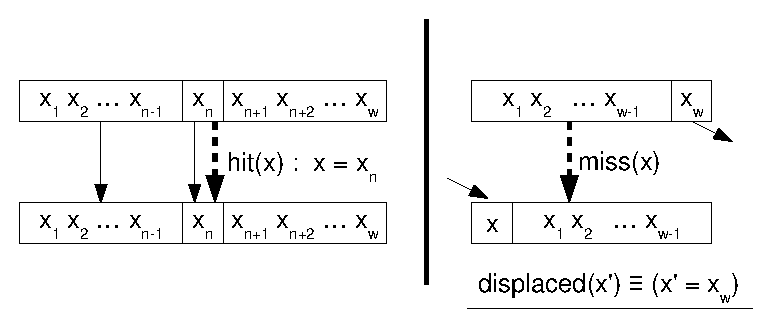
\includegraphics[width=0.6\textwidth]{2.theor/fifo1}\\
  \caption{Стратегия вытеснения \FIFO (w --- ассоциативность
таблицы)}\label{fifo1}
\end{figure}

Отличие от \LRU лишь в том, что при \FIFO не происходит перестановки
элементов региона при возникновении попадания. Поэтому таблица
вытеснения~\cite{policy_tables} для стратегии вытеснения \FIFO будет
выглядеть так, как изображено на рисунке~\ref{fifo_policy_table}.

\begin{figure}
$$
  \left[
    \begin{array}{c|cccccc}
      \pi_0 & 0 & 1 & 2 & 3 & \dots & w-1 \\
      \pi_1 & 0 & 1 & 2 & 3 & \dots & w-1 \\
      \pi_2 & 0 & 1 & 2 & 3 & \dots & w-1 \\
      \vdots &  &  &  & & & \\
      \pi_{w-1} & 0 & 1 & 2 & 3 & \dots & w-1 \\
      \pi_m & m & 0 & 1 & 2 & \dots & w-2 \\
    \end{array}
  \right]
$$
\caption{Таблица вытеснения для \FIFO}\label{fifo_policy_table}
\end{figure}

Стратегия вытеснения \FIFO есть частный случай
\LRU, в котором попадание не меняет состояния вектора.
Поэтому и ограничения с функциями полезности для \FIFO будем строить
на основе уже сформулированных и обоснованных ограничений с
функциями полезности для \LRU. %Кроме того все инструкции с
%попаданиями, поскольку они не влияют на вытеснение, можно вообще
%исключить из ограничений.

Таким образом система уравнений для описания обращений по ключу $k$ в регион $R$
согласно методу функций полезности для \FIFO выглядит следующим образом:
\begin{itemize}
\item $k$ еще не вытеснен из региона $R$:
$$
\left\{\begin{array}{l} (k||R) \in \{(t_1||r_1), ..., (t_m||r_m), (k_1||R_1),
..., (k_n||R_n)\}\\
\sum\limits_{i=1}^m u_{k,R}(t_i||r_i) + \sum\limits_{i=1..n:(k_i,R_i)\mbox{~--
miss}} u_{k,R}(k_i||R_i) < w\\
\{(t_1||r_1), ..., (t_m||r_m)\} - \mbox{все разные}\\
\end{array} \right.
$$
\item $k$ вытеснен из региона $R$:
$$
\left\{\begin{array}{l} (k||R) \in \{(t_1||r_1), ..., (t_m||r_m), (k_1||R_1),
..., (k_n||R_n)\}\\
\sum\limits_{i=1}^m u_{k,R}(t_i||r_i) + \sum\limits_{i=1..n:(k_i,R_i)\mbox{~--
miss}} u_{k,R}(k_i||R_i)
\geqslant w\\
\{(t_1||r_1), ..., (t_m||r_m)\} - \mbox{все разные}\\
\end{array} \right.
$$
\end{itemize}

$$u_{k,R}(s_i) \equiv ((k||R) \notin \{s_i, ..., s_{m+n}\} \wedge
R = R(s_i) \wedge s_i \notin\{s_{i+1},..., s_{m+n}\})$$
$s \equiv \langle (t_1||r_1), ..., (t_m||r_m), (k_1||R_1), ...,
(k_n||R_n)\rangle$, $R(s_i)$ --- вторая компонента $s_i$ (регион).


\subsection{Метод функций полезности для стратегии вытеснения \PseudoLRU}

Для выделения функционала вытеснения воспользуемся определением\\\PseudoLRU <<на
ветвях бинарного дерева>> (см. раздел~\ref{sec:PseudoLRUonBranches}). А именно,
определение того, вытеснен ли ключ $k$ в регионе $R$, будет вестись на основе
атрибутов вершин пути от корня дерева к соответствующему ключу листу. Эти
вершины могут быть белыми (им сопоставлено число 0) или чёрными (им сопоставлено
число 1). Обращение по другому ключу $k_i$ (в этом же регионе) перекрашивает
некоторые вершины этого пути. А именно, при следовании от корня к листу сначала
часть вершин перекрашивается в белый цвет, затем одна вершина красится в черный
цвет, остальные вершины не перекрашиваются. Если происходит обращение к листу,
то вся ветвь красится в белый цвет.

\begin{figure}[h] \center
  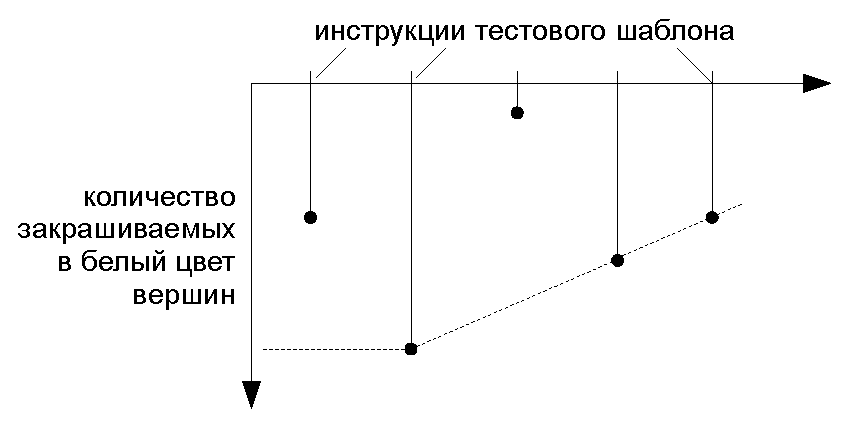
\includegraphics[width=0.6\textwidth]{2.theor/white_feeds}
  \caption{Последовательность закрашиваний белыми вершинами и ее выпуклая
оболочка}\label{fig:white-feeds}
\end{figure}

На рисунке~\ref{fig:white-feeds} изображена последовательность из
чисел-количеств вершин некоторой ветви, которые закрашивается в белый цвет
очередной инструкцией тестового шаблона. Пунктиром обозначена ее <<выпуклая
оболочка>>. Количество различных элементов в этой последовательности, которые
входят в границу <<выпуклой оболочки>> соответствует количеству черных вершин в
ветви. Вытеснение произойдет тогда, когда вся ветвь будет черной, т.е. когда
количество различных инструкций, попадающих в границу <<выпуклой оболочки>>,
превысит некоторую константную границу. Верно и обратное, вытеснение не
произойдет, если количество этих инструкций будет меньше. Перекрашивание
выполняется лишь на основе самой ветви. При обращении по тому ключу, который
соответствует листу рассматриваемой ветви, количество черных вершин становится
минимальным (равным 0). Итак, для стратегии вытеснения \PseudoLRU \emph{в
качестве функционала вытеснения рассмотрим длину <<нижней>> черной части} пути к
листу.

%Например, представленный на рисунке~\ref{fig:plru-useful} шаблон успевает
% покрасить 5 вершин ветви в черный цвет.
%
%\begin{figure}[t] \center
%  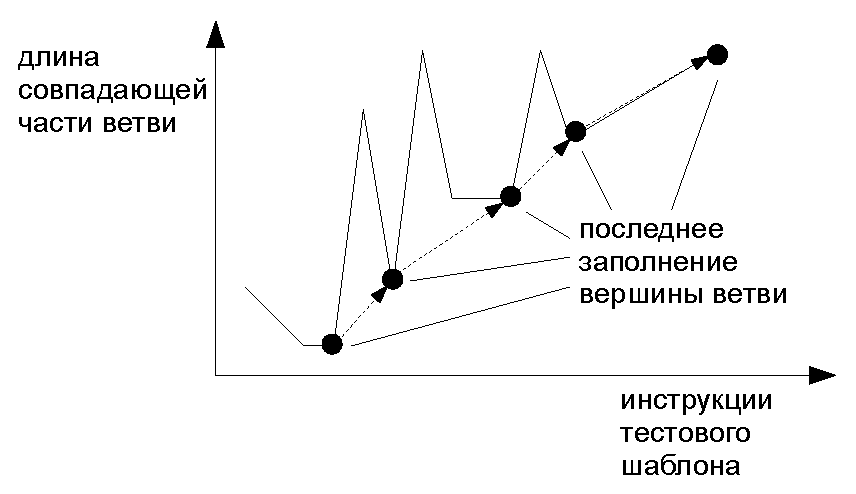
\includegraphics[width=0.6\textwidth]{2.theor/plru-useful}\\
%  \caption{Заполнение ветви черными вершинами в стратегии вытеснения
%  \PseudoLRU}\label{fig:plru-useful}
%\end{figure}

\begin{utv}
Инструкция $I$ считается полезной в случае стратегии вытеснения
\PseudoLRU, если все последующие инструкции затрагивают только те
вершины ветви, которые расположены выше вершины, перекрашиваемой инструкцией $I$
в черный цвет.
\end{utv}

Для вытеснения нужно не менее $\log_2 w$ полезных инструкций (длина ветви).
Далее выражение $\log_2 w$ будет обозначаться буквой $W$.

Отличие этого функционала вытеснения от функционала для \LRU является \emph{немонотонность}. Это означает, что полезные инструкции надо считать для каждого промаха заново ---
инструкции между двумя соседними промахами могут <<забелить>>
несколько вершин ветви, что уменьшит функционал вытеснения
(см.рис.~\ref{nonmonotonic}). Метрика для \LRU является монотонной,
потому что инструкции между промахами не могут уменьшить функционал вытеснения -- либо не меняют, либо увеличивают ее, сдвигая ключ к концу вектора \LRU (см. рис.~\ref{monotonic}).

%Таким образом, ограничение, описывающее стратегию вытеснения
%\PseudoLRU, будет представлено дизъюнкцией ограничений по всем
%предыдущим кэш-промахам.

\begin{figure}[h] \center
  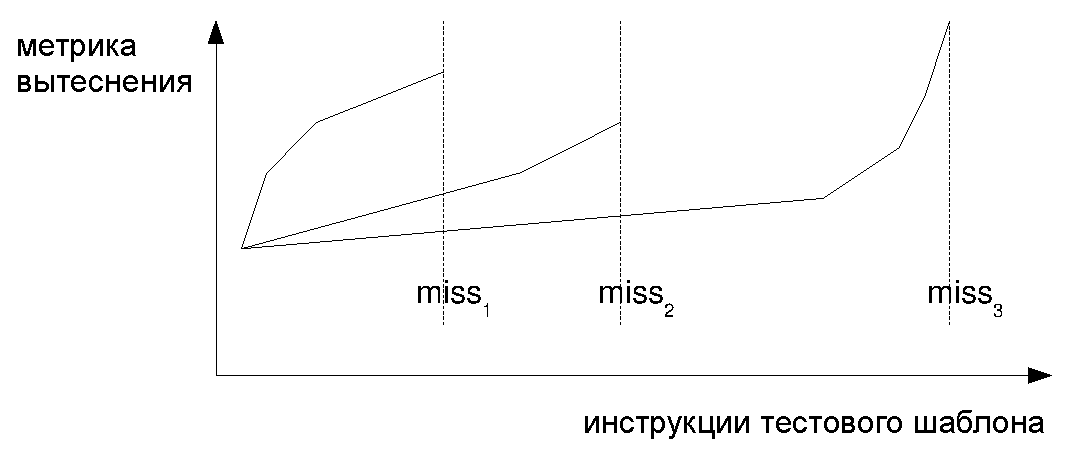
\includegraphics[width=0.6\textwidth]{2.theor/nonmonotonic}\\
  \caption{Немонотонный функционал вытеснения}\label{nonmonotonic}
\end{figure}

\begin{figure}[h] \center
  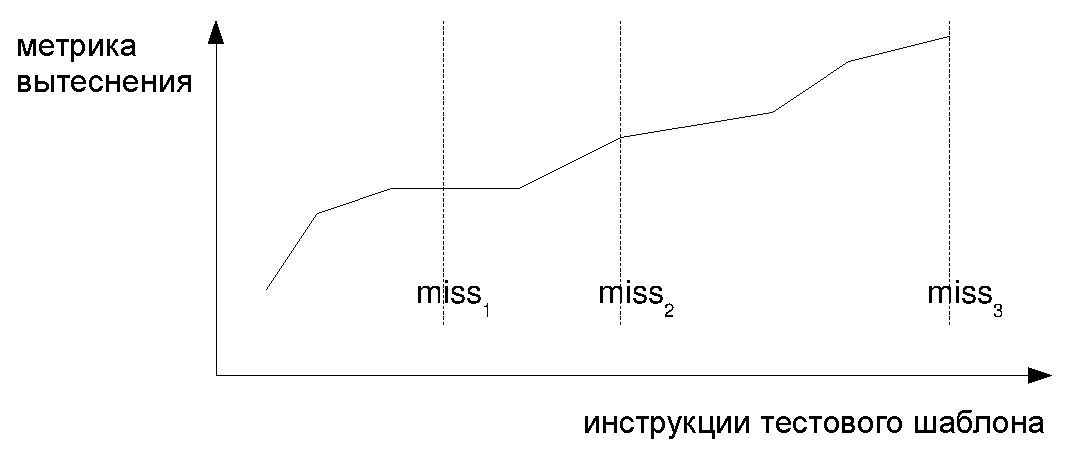
\includegraphics[width=0.6\textwidth]{2.theor/monotonic}\\
  \caption{Монотонный функционал вытеснения}\label{monotonic}
\end{figure}

Осталось записать понятие полезной инструкции для \PseudoLRU в виде
ограничений. Каждый ключ $k_i$ в регионе $R_i$ кроме своего значения
снабжен <<позицией>> $\pi_i$ ($\pi_i \in \{0..w{-}1\})$. Позиции -- это еще один
набор переменных в добавление к ключам и регионам. Пусть надо записать
ограничение, что ключ $k$ в регионе $R$ вытеснен в некоторой инструкции. Пусть
$(k_1, R_1)$, $(k_2, R_2)$, ..., $(k_n, R_n)$ --- ключи и регионы предыдущих
инструкций. Надо выяснить, когда заданная предыдущая инструкция будет полезной
для вытеснения ключа $k$ из региона $R$. Инструкция не может быть полезной, пока
не произошло в последний раз обращение к ключу $k$ в регионе $R$. В момент этого
последнего обращения ветвь к нему становится целиком белой и начинается процесс
вытеснения. Т.е. для дальнейших инструкций нам будет важно, каким позициям
соответствуют в них ключи. Согласно определению полезные инструкции должны
закрашивать больше белых вершин, чем закрашивают все последующие инструкции. И,
наконец, эта логика в виде ограничений -- $(k_i, R_i, \pi_i)$ будет полезным для
вытеснения ключа $k$ в регионе $R$, если выполнены все следующие условия:
\begin{itemize}
    \item $(k||R) \notin \{(k_i||R_i), (k_{i+1}||R_{i+1}), ..., (k_n||R_n)\}$ --
инструкция расположена после последнего обращения к $k$ в $R$;
    \item $R = R_i$ -- инструкция обращатеся в тот же регион;
    \item $P(\pi_i \oplus \pi,~\pi_{i+1} \oplus \pi) \wedge P(\pi_i \oplus
\pi,~\pi_{i+2} \oplus \pi) \wedge ... \wedge P(\pi_i \oplus \pi,~\pi_{n-1}
\oplus \pi)$ -- все последующие обращения должны пересекаться только в более
верхних частях ветви (это выражает предикат $P$ для пары векторов); обращение в
$n$'й инструкции должно быть промахом (потом это условие будет обеспечено);
предикат $P(\delta_i, \delta_j)$ истинен тогда и только тогда, когда количество
старших нулевых бит у $\delta_i$ больше количества старших нулевых бит у
$\delta_j$, иными словами, только и только тогда, когда существует $k$ такое,
что $\delta_i < 2^k \leqslant \delta_j$; с использованием битовых операций этот
предикат записывается в следующем виде: $P(\delta_i, \delta_j) \equiv
(\delta_j > \delta_i~~\wedge~~\delta_j \oplus \delta_i > \delta_i)$, сравнения
беззнаковые.
\end{itemize}

Итак, система уравнений для описания обращений по ключу $k$ в регион $R$
согласно методу функций полезности для \PseudoLRU:
\begin{itemize}
\item $k$ еще не вытеснен из региона $R$:
$$
\left\{\begin{array}{l}
(k||R) \in \{(t_1||r_1), ..., (t_m||r_m), (k_1||R_1), ..., (k_n||R_n)\}\\
\{(t_1||r_1), ..., (t_m||r_m)\} - \mbox{все разные}\\
\bigvee_{q:1..n:\mbox{miss}} \sum\limits_{i=1}^m u_{k,R}(t_i||r_i) +
\sum\limits_{i=1}^q u_{k,R}(k_i||R_i) < W\\
\end{array} \right.
$$
\item $k$ вытеснен из региона $R$:
$$
\left\{\begin{array}{l} (k||R) \in \{(t_1||r_1), ..., (t_m||r_m), (k_1||R_1),
..., (k_n||R_n)\}\\
\{(t_1||r_1), ..., (t_m||r_m)\} - \mbox{все разные}\\
\bigwedge_{q:1..n:\mbox{miss}} \sum\limits_{i=1}^m u_{k,R}(t_i||r_i) +
\sum\limits_{i=1}^q u_{k,R}(k_i||R_i) \geqslant W\\
\end{array} \right.
$$
\end{itemize}

$$u_{k,R} (s_i) \equiv \left\{\begin{array}{l}
(k||R) \notin \{(k_i||R_i), (k_{i+1}||R_{i+1}), ..., (k_n||R_n)\}\\
R = R(s_i)\\
P(\pi_i \oplus \pi,~\pi_{i+1} \oplus \pi)\\
P(\pi_i \oplus \pi,~\pi_{i+2} \oplus \pi)\\
... \\
P(\pi_i \oplus \pi,~\pi_{n-1} \oplus \pi)
\end{array}\right.
$$
$$s \equiv \langle (t_1,r_1), (t_2,r_2), ..., (t_m,r_m), (k_1, R_1), ...,
(k_n,R_n) \rangle$$
$$R(s_i) \mbox{~--- вторая компонента~} s_i$$

Поскольку введены позиции, то надо еще в систему ограничений включить
соотношение позиций и ключей --- конъюнкцию для каждой пары $(s_i,\pi_i)$ и
$(s_j, \pi_j)$, где инструкция второй пары расположена после инструкции первой
пары, ограничений:
\begin{itemize}
    \item если вторая инструкция --- попадание, то $$(\pi_i||R(s_i) =
\pi_j||R(s_j)~\wedge$$ $$\pi_i||R(s_i) \notin \{\pi_{m_1}||R(s_{m_1}),
\pi_{m_2}||R(s_{m_2}), \dots, \pi_{m_n}||R(s_{m_n})\}) \rightarrow s_i = s_j$$
    \item если вторая инструкция --- промах, то $$(\pi_i||R(s_i) =
\pi_j||R(s_j)~\wedge$$ $$\pi_i||R(s_i) \notin \{\pi_{m_1}||R(s_{m_1}),
\pi_{m_2}||R(s_{m_2}), \dots, \pi_{m_n}||R(s_{m_n})\}) \rightarrow s_i \neq
s_j$$
\end{itemize}
где $(\pi_{m_1},R(s_{m_1})), (\pi_{m_2},R(s_{m_2})), \dots,
(\pi_{m_n},R(s_{m_n}))$ --- позиции и регионы\\инструкций-промахов,
расположенных между $i$'й и $j$'й инструкциями. В качестве $i$'й инструкции
также надо рассмотреть и инициализирующие инструкции.

%Таблица~\ref{plru_table} содержит ограничения для разных случаев
%кэш-попаданий и кэш-промахов (см. утверждение~\ref{hit_miss_human}).
%В каждое из них включается ограничение на количество полезных
%инструкций согласно предлагаемой методике использования функций
%полезности. Полезности считаются относительно некоторого кэш-промаха
%(для их перебора используется сокращение $x_m : \mbox{miss}$).

Нетрудно заметить, что построение формул в точности повторяло записанное при них неформально, а оно напрямую следовало из определения \PseudoLRU на ветвях бинарного дерева. Из чего следует и обоснование приведенных формул.


\subsection{Разрешение уравнений, описывающих стратегии вытеснения}

Ограничения, которые предлагается генерировать для описания тестовых ситуаций,
являются \emph{ограничениями мощности} (cardinality constraints). Это
ограничения вида $C_1 \leqslant \sum_{i=1}^n a_i \leqslant C_2$, где $C_1, C_2$
-- неотрицательные целые числа, а $a_i$ принимают значения 0 или
1~\cite{smt_debugging, PiskacK08, KuncakR07,
Revesz05}. Речь идет об ограничении размера некоторого множества
элементов, заданного с помощью характеристической функции.
В~\cite{smt_debugging} проведено исследование способов записи
ограничений мощности и показано, что от формы записи зависит
эффективность разрешения этих ограничений. Одна из таких форм рассматривает ограничения
мощности как компактную форму записи уравнения
вида $\bigvee_{C_1 \leqslant C \leqslant C_2} \sum_{i=1}^n a_i = C$,
где равенство есть
\begin{itemize}
\item тождественная ложь, если $C < 0$ или $C > n$;
\item конъюнкция $\bigwedge_{1\leqslant i\leqslant n} (a_i = 0)$,
если $C = 0$;
\item дизъюнкция по всевозможным выборкам индексов $i_1, ..., i_C$, где
для каждого индекса $i_k$ справедливы свойства $1 \leqslant i_k
\leqslant n$ и $i_k < i_{k+1}$, конъюнкций $\bigwedge_{i_k} (a_{i_k}
= 1)$, если $1 \leqslant C \leqslant n$.
\end{itemize}

В данной работе не ставилась задача исследования способов разрешения ограничений
мощности (с целью выбора наиболее эффективного способа их представления). Вместо
этого были использованы
имеющиеся инструменты разрешения ограничений мощности~\cite{Z3, Yices}. Для
записи оставшихся формул были использован язык битовых строк, для разрешения
формул над которым существуют эффективные SMT-инструменты (например,
Z3~\cite{Z3}).

%После устранения ограничений мощности в формуле остаются только
%ограничения на конечные множества тегсетов: принадлежности и
%непринадлежности тега конечному множеству тегсетов и равенства и
%неравенства битовых полей тегсетов. Поскольку конечные множества
%тегсетов известны (заданы перечислением тегсетов, которые в входят в
%это множество), то ограничения принадлежности и непринадлежности
%могут быть переписаны без использования этих отношений. Отношение
%принадлежности $x \in \{x_1, x_2, ..., x_n\}$ может быть переписано
%в виде дизъюнкции $(x = x_1) \vee (x = x_2) \vee ... \vee (x =
%x_n)$, а отношение непринадлежности $x \notin \{x_1, x_2, ...,
%x_n\}$ -- в виде конъюнкции $(x \neq x_1) \wedge (x \neq x_2) \wedge
%... \wedge (x \neq x_n)$.
%
%В результате получается предикат, в котором переменными величинами
%являются неотрицательные целые числа с конечной областью значений
%(тегсеты), над переменными возможны операции получения битового
%поля, в предикате используется отношение равенства и неравенства над
%битовыми полями. Кроме того, этот предикат задается с использованием
%ограничений мощности.
%
%Для разрешения такого рода предикатов можно было бы разрабатывать
%собственные процедуры распространения ограничений, но это свело бы
%на нет все усилия по выработке собственного представления стратегии
%вытеснения. Однако предлагаемые ограничения могут быть тривиальным
%образом выражены на языке теорий, для которых существуют эффективные
%разрешающие процедуры (битовые строки, неинтерпретируемые функции).
%Поэтому для записи и разрешения этих ограничений могут быть
%использованы SMT-инструменты~\cite{Z3}.

%%%%%%%%%%%%%%%%%%%%%%%%%%%%%%%%%%%%%%%%%%%%%%%%%%%%%%%%%%%%%%%%%%%
%
%\pagebreak
%\section{Ограничения, описывающие тестовые ситуации в некоторых
%частных случаях, для стратегии вытеснения \LRU}
%
%\subsection{Тестовые шаблоны без кэш-промахов}
%
%В случае тестовых шаблонов, в которых нет кэш-промахов, нет ни
%вытесняющих, ни вытесняемых тегсетов. Поэтому в таких шаблонов
%уравнения для кэш-попаданий имеют очень простой вид:
%
%$$
%\left\{
%\begin{array}{l}
%x \in D\\
%... (\mbox{тестовые ситуации на остальные буферы})\\
%\end{array}
%\right.
%$$
%
%\subsection{Тестовые шаблоны без кэш-попаданий}
%
%В случае тестовых шаблонов, в которых нет кэш-попаданий, надо
%генерировать ограничения для вытесняющих и лишь иногда для
%вытесняемых тегсетов. А именно, вытесняемый тегсет требуется лишь в
%том случае, когда кэш-промах вносит в кэширующий буфер ранее
%вытесненный тегсет. В этом случае для вытесняемого тегсета известен
%домен, что позволяет построить уравнения обозримого размера. Кроме
%того, поскольку отсутствуют кэш-попадания, повторные обращения к
%вытесняемым тегсетам (кроме кэш-промаха, который их может внести в
%кэширующий буфер) невозможны, что также упрощает генерируемые
%уравнения.
%
%В результате получается, что вытесняющий тегсет описывается в
%тестовом шаблоне без кэш-попаданий следующей системой уравнений:
%$$
%F'(x) \vee F''(x) \vee \bigvee_{\lambda_\delta \in D} F'''(x, \lambda_\delta)
%$$
%
%где
%
%$$F'(x) \equiv (x \notin D \wedge x \notin \{x_1, ..., x_n\})$$
%
%$$F''(x) \equiv (x \in \{x_1, ..., x_n\} \wedge \sum_{i=1}^n u''(x_i) \geqslant w)$$
%
%$$u''(x_i) \equiv (x\notin \{x_i, ..., x_n\} \wedge R(x_i) = R(x))$$
%
%$$F'''(x, \lambda_\delta) \equiv (x = \lambda_\delta \wedge x \notin
%\{x_1, ..., x_n\} \wedge \sum_{i=1}^n (R(x_i) = R(x)) \geqslant w -
%\delta + 1)$$
%
%\subsection{Короткие тестовые шаблоны}
%
%Будем называть тестовый шаблон \emph{коротким}, если в нем не более
%$w$ инструкций обращения к памяти. Очевидно, что любой короткий
%тестовый шаблон является простым. Из 7 случаев для коротких тестовых
%шаблонов остается всего 5 (первые два можно еще объединить в более
%компактную систему уравнений). В таблице~\ref{short_templates_table}
%предъявлены функции полезности и ограничения для коротких тестовых
%шаблонов в случае стратегии вытеснения \LRU. Соответствующая теорема
%корректности этих ограничений сформулирована и доказана в
% приложении~\ref{sec:proofs}.
%
%\begin{table}[t]
%\begin{tabular}{|c|c|c|c|}
%\hline  & \centering случай &
%\begin{tabular}{c}переменная\\перебора\end{tabular} & система \\
%\hline \hline \multirow{-2}{*}{\rotatebox{90}{кэш-попадание}} &
%\makecell[c{p{0.3\textwidth}}]{тегсет находится в начальном
%состоянии буфера и он всё ещё не вытеснен} & $\lambda_\delta \in D$
%&
%$\left\{\begin{array}{l} x = \lambda_\delta\\
%\sum\limits^n_{i=1} u(x_i) \leqslant w - \delta
%\end{array}\right.$ \\ \hhline{~|---}
%& \makecell[c{p{0.3\textwidth}}]{тегсет уже встречался в шаблоне} &
%-- & $x \in \{x_1, ..., x_n\}$
%\\ \hline \hline \multirow{6}{*}{\rotatebox{90}{кэш-промах}}
%& \makecell[c{p{0.3\textwidth}}]{тегсет встречается впервые} & -- &
%$\left\{\begin{array}{l} x \notin D\\
%x \notin \{x_1, ..., x_n\}\\
%\end{array}\right.$\\ \hhline{~|---} &
%\makecell[c{p{0.3\textwidth}}]{тегсет находился в начальном
%состоянии буфера и был вытеснен} & $\begin{array}{c}\lambda_\delta
%\in D,\\\delta \geqslant w-n+1\end{array}$ &
%$\left\{\begin{array}{l} x = \lambda_\delta\\
%x \notin \{x_1, ..., x_n\}\\
%\sum\limits^n_{i=1} u(x_i) > w - \delta\\
%\end{array}\right.
%$ \\ \hline
%\end{tabular}
%
%%где функция полезности определена следующим образом:
%$$u(x_i) \equiv
%\left\{\begin{array}{l} x_i \in \{ \lambda_{\delta+1}, ...,
%\lambda_w\}~\wedge~x_i \notin \{x_1, ..., x_{i-1}\}, \mbox{если}~S_i
%= \mbox{hit}\\
%R(x_i) = R(x), \mbox{если}~S_i = \mbox{miss}
%\end{array}\right.
%$$
%\caption{Таблица систем уравнений для тестовых ситуаций в кэширующих
%буферах для коротких тестовых шаблонов в случае стратегии вытеснения
%\LRU}\label{short_templates_table}
%\end{table}
%
%
%
%%\begin{landscape}
%%\begin{table}
%%\begin{tabular}{|c|c|c|c|c|c|}
%%\hline  & \centering случай &
%%\begin{tabular}{c}переменная\\перебора\end{tabular} & система &
%%\begin{tabular}{c}функция\\полезности\\для кэш-\\попадания\end{tabular} &
%%\begin{tabular}{c}функция\\полезности\\для кэш-\\промаха\end{tabular} \\
%%\hline \hline \multirow{-2}{*}{\rotatebox{90}{кэш-попадание}} &
%%\makecell[c{p{0.3\textwidth}}]{тегсет находится в начальном
%%состоянии буфера и он всё ещё не вытеснен} & $\lambda_\delta \in
%%D$ &
%%$\left\{\begin{array}{l} x = \lambda_\delta\\
%%\sum\limits^n_{i=1} u(x_i) \leqslant w - \delta
%%\end{array}\right.
%%$ &
%%\begin{tabular}{c}
%%$x_i \in \{ \lambda_{\delta+1}, ..., \lambda_w\}$\\
%%$\wedge~x_i \notin \{x_1, ..., x_{i-1}\}$
%%\end{tabular}
%%& $R(x_i) = R(x)$
%%\\ \hhline{~|-----}
%%& \makecell[c{p{0.3\textwidth}}]{тегсет уже встречался в шаблоне} &
%%-- & $x \in \{x_1, ..., x_n\}$ & -- & --
%%\\ \hline \hline \multirow{6}{*}{\rotatebox{90}{кэш-промах}}
%%& \makecell[c{p{0.3\textwidth}}]{тегсет встречается впервые} & -- &
%%$\left\{\begin{array}{l} x \notin D\\
%%x \notin \{x_1, ..., x_n\}\\
%%\end{array}\right.
%%$ & -- & -- \\ \hhline{~|-----} &
%%\makecell[c{p{0.3\textwidth}}]{тегсет находился в начальном
%%состоянии буфера и был вытеснен} &
%%$\begin{array}{c}\lambda_\delta \in D,\\\delta \geqslant
%%w-n+1\end{array}$ &
%%$\left\{\begin{array}{l} x = \lambda_\delta\\
%%x \notin \{x_1, ..., x_n\}\\
%%\sum\limits^n_{i=1} u(x_i) > w - \delta\\
%%\end{array}\right.
%%$ &
%%\begin{tabular}{c}
%%$x_i \in\{\lambda_{\delta+1}, ..., \lambda_w\}$\\
%%$\wedge~x \notin \{x_1, ..., x_{i-1}\}$\\
%%\end{tabular}
%%&
%%\begin{tabular}{c}
%%$R(x_i) = R(x)$\\
%%\end{tabular}
%%\\ \hline
%%\end{tabular}
%%\caption{Таблица систем уравнений для тестовых ситуаций в кэширующем буфере
%%для коротких тестовых шаблонов в случае стратегии вытеснения
%%\LRU}\label{short_templates_table}
%%\end{table}
%%\end{landscape}
%
%
%\subsection{Генерация тестовых данных для кэш-памяти, содержащей
%<<грязные>> ячейки}
%
%Любая ячейка в кэш-памяти может быть помечена \emph{грязной}
%(\emph{invalid}). Это означает, что данные, находящиеся в кэширующем
%буфере по этому адресу, не могут использоваться в качестве данных,
%хранящихся в памяти по этому адресу.
%
%Рассмотренные ранее в этой работе случаи не учитывали грязные ячейки
%кэширующем буфере, хотя они зачастую присутствуют в микропроцессоре
%после его запуска -- с таким состоянием кэширующего буфера работают
%первые после запуска микропроцессора инструкции.
%
%Кэш-попадание возникает в том случае, когда требуемые данные
%присутствуют среди <<чистых>> ячеек кэширующего буфера. Кэш-промах
%возникает в том случае, когда требуемых данных нет среди <<чистых>>
%ячеек. Причем при наличии <<грязных>> ячеек вытеснения может и не
%произойти. А именно, если все ячейки набора, с которым работает
%инструкция, являются <<чистыми>>, то происходит вытеснение согласно
%стратегии вытеснения, остальные наборы не меняются. Если же среди
%ячеек набор есть <<грязные>> ячейки, то вытеснение не происходит, а
%на место одной из <<грязных>> ячеек помещаются данные из основной
%памяти по заданному адресу и ячейка объявляется <<чистой>>.
%Остальные ячейки не меняются. В стратегии вытеснения \LRU эта бывшая
%<<грязная>> ячейка становится самой новой.
%
%Для генерации тестовых данных для кэширующих буферов с грязными
%ячейками предлагается применять ограничения с функциями полезности.
%Примечательно, что наличие грязных ячеек не меняет качественно
%систему уравнений.
%
%В данном разделе рассматривается случай, когда начальное состояние
%микропроцессора известно. Кроме того, рассматриваемый случай
%учитывает отсутствие инструкций в тестовом шаблоне, которые
%превращали бы <<чистые>> ячейки в <<грязные>> (т.е. все такие
%изменения должны делаться явно вне тестовых шаблонов).
%
%\subsubsection{случай полностью-ассоциативного кэширующего буфера}
%
%В случае полностью-ассоциативных кэширующих буферов очевидно, что
%первые кэш-промахи будут заполнять <<грязные>> ячейки. Пусть $N$ --
%количество <<грязных>> ячеек в начальном состоянии кэширующего
%буфера, а $L_0$ -- начальное состояние (выражение) кэширующего
%буфера (только <<чистые>> ячейки). Тогда для тестовых ситуаций надо
%генерировать такие ограничения ($L$ -- выражение для состояния
%кэширующего буфера перед исполнением инструкции, $L'$ -- выражение
%для состояния кэширующего буфера после исполнения инструкции):
%\begin{itemize}
%\item для \emph{кэш-попадания} hit($x$) генерируются ограничения
%$$
%\left\{
%\begin{array}{l}
%x \in L\\
%L' \equiv L\\
%\end{array}
%\right.
%$$
%
%\item для \emph{кэш-промаха} miss($x$), если это один из первых $N$
%кэш-промахов, генерируются ограничения:
%$$
%\left\{
%\begin{array}{l}
%x \notin L\\
%L' \equiv L \cup \{x\}\\
%\end{array}
%\right.
%$$
%
%\item для \emph{кэш-промаха} miss($x$), являющегося по счету более
%чем $N$'м кэш-промахом тестового шаблона, генерируются ограничения:
%$$
%\left\{
%\begin{array}{l}
%x \notin L\\
%x' \in L\\
%L' \equiv L\setminus\{x'\} \cup \{x\}\\
%displaced(x', L)\\
%\end{array}
%\right.
%$$
%\end{itemize}
%
%Предикат $displaced(x', L)$ истинен, если $x'$ является вытесняемым
%тегом в текущем состоянии кэширующего буфера $L$. Для стратегии
%вытеснения \LRU этот предикат может быть записан с использованием
%тех же диапазонов вытеснения, что и для кэширующего буфера без
%<<грязных>> ячеек (см.п.~\ref{LRU_constraints}). А именно, диапазон
%вытеснения начинается на инструкции, которая последний раз перед
%вытеснением тега обращается к нему. Тогда между этой инструкцией и
%инструкцией, вытесняющей $x$, должны быть обращения ко всем
%остальным тегам текущего состояния кэширующего буфера. Эта логика
%может быть записана в виде тех же уравнений, что и в
%пункте~\ref{LRU_constraints}. Нетрудно проверить, что для
%кэширующего буфера с <<грязными>> ячейками остается справедливой
%лемма о невложенных диапазонах вытеснения, что доказывает
%корректность использования ограничений из
%пункта~\ref{LRU_constraints} для кэширующего буфера с <<грязными>>
%ячейками.
%
%\subsubsection{случай наборно-ассоциативного кэширующего буфера}
%
%В этом пункте будет показано, что ограничения для кэширующего
%буфера, начальное состояние которого содержит <<грязные>> ячейки,
%качественно не отличаются от ограничений для кэширующего буфера без
%<<грязных>> ячеек.
%
%Аналогично тому, как это делалось для кэширующих буферов без
%<<грязных>> ячеек, для тестовых ситуаций на кэширующие буферы с
%<<грязными>> ячейками тоже возможно следующее исчерпывающее
%выделение случаев:
%\begin{itemize}
%\item кэш-попадание тега:
%    \begin{enumerate}
%    \item данный тег находился в начальном состоянии кэширующего буфера и не был
%    вытеснен к моменту данной инструкции;
%    \item данный тег был внесен в кэширующий буфер одной из инструкций
%    кэш-промаха и с тех пор не был вытеснен;
%    \end{enumerate}
%\item кэш-промах тега:
%    \begin{enumerate}
%    \item данный тег не встречался ранее (не находился в начальном
%    состоянии кэширующего буфера и не был внесен какими-либо кэш-промахами);
%    \item данный тег был ранее вытеснен из кэширующего буфера и с тех пор
%    не был внесен в кэширующий буфер вновь.
%    \end{enumerate}
%\end{itemize}
%
%Соответствующие ограничения приведены в
%таблице~\ref{dirty_hit_miss_table}.
%
%
%В таблице~\ref{dirty_hit_miss_table} символ $\Delta$ означает
%количество <<чистых>> ячеек в начальном состоянии того региона, про
%который идет речь в уравнении. На самом деле $\Delta$ есть функция
%региона ($\Delta = \Delta(\lambda_\delta)$), но для сокращения
%записи оставлен только функциональный символ. Кроме того, в
%приведенных уравнениях домен переменной включает только <<чистые>>
%ячейки.
%
%Сходства уравнений (со случаем кэширующих буферов без <<грязных>>
%ячеек) удалось добиться за счет рассмотрения <<грязных>> ячеек, как
%ячеек с наименьшим счетчиком \LRU, которые не участвуют в
%определении нахождения тега в кэширующих буферах. Поэтому в функциях
%полезности участвуют множества не $\{\lambda_{\delta+1}, ...,
%\lambda_w\}$, а множества $\{\lambda_{\delta+1}, ...,
%\lambda_\Delta\}$. Все <<чистые>> ячейки получили первые индексы,
%т.е. индексы всех от 1 до $\Delta$.
%
%%\begin{theorem}[корректность использования функций полезности для
%%записи \LRU в случае наличия <<грязных>> ячеек в начальном состоянии
%%кэширующего буфера] Тестовая программа, построенная по ограничениям,
%%которые сгенерированы с использованием предъявленных в
%%таблице~\ref{dirty_hit_miss_table} функций полезности, в случае
%%наличия <<грязных>> ячеек в начальном состоянии кэширующего буфера
%%удовлетворяет своему тестовому шаблону.
%%\end{theorem}
%%\begin{proof}
%%  //TODO
%%\end{proof}
%
%Для приведенных ограничений также могут быть применены эвристики,
%сокращающие их количество, которые были упомянуты для кэширующих
%буферов без <<грязных>> ячеек. Кроме того, в данном случае возможна
%дополнительная эвристика \emph{ограничение на $\delta$}: если
%$\delta + 1 < \Delta$, то функция полезности, в которую входит
%множество $\{\lambda_{\delta+1}, ..., \lambda_\Delta\}$, равна 0.
%
%%\subsection{Функции полезности для зеркальной генерации тестовых
%%данных}
%%
%%Рассмотрим ограничения, генерируемые для тестовых шаблонов
%%зеркальным методом с использованием функций полезности. По сравнению
%%с представленными ограничениями (см. табл.~\ref{hit_miss_table})
%%зеркальная генерация имеет свои особенности:
%%\begin{enumerate}
%%  \item множества констант (как, например, $L, D$) не используются,
%%  поэтому в ограничениях будут отсутствовать соответствующие им
%%  случаи;
%%  \item так как теги инструкций тестового шаблона должны появиться
%%  среди инициализирующей последовательности, то для вытеснения
%%  требуется $w-1$ инструкций, где $w$ -- ассоциативность кэширующего буфера;
%%  \item учет полезных инструкций начинается уже в инициализирующей
%%  последовательности, тем самым необходимо сформулировать функцию
%%  полезности для инициализирующих инструкций.
%%\end{enumerate}
%%
%%Следующая теорема описывает функцию полезности для инициализирующих
%%инструкций и описывает ограничения, генерируемые для тестовых
%%шаблонов зеркальным методом с использованием функций полезности
%%(количество инициализирующих инструкций зафиксировано, оно будет
%%обозначено параметром $m$):
%%
%%\begin{theorem}[Корректность ограничений, генерируемые зеркальным методом с
%%использованием функций полезности для
%%\LRU]\label{correct_mirror_LRU} Пусть $t_1, t_2, ..., t_m$ -- теги
%%инициализирующей последовательности, $x$ -- текущий тег тестового
%%шаблона, $x_1, x_2, ..., x_n$ -- теги предыдущих инструкций
%%тестового шаблона, причем $x \in \{t_1, ..., t_m, x_1, ..., x_n\}$ и
%%$\{t_1, ..., t_m\}$ --- все разные. Тогда $x$ не вытеснен согласно
%%определению на списках тогда и только тогда, когда
%%$$\sum\limits_{i=1}^{m+n} u_x(s_i) < w$$
%%где последовательность $s \equiv \langle t_1, ..., t_m, x_1, ...,
%%x_n\rangle$, а функция полезности определена следующим образом:
%%$$u_x(s_i) \equiv (x \notin \{s_i, ..., s_{m+n}\} \wedge
%%R(x) = R(s_i) \wedge s_i \notin\{s_{i+1},..., s_{m+n}\})$$
%%
%%%$$\sum\limits_{i=1}^m \tilde{u}_x(t_i) + \sum\limits_{i=1}^n u_x(x_i) < w$$
%%%где функции полезности определены следующим образом:
%%%$$\begin{array}{c}
%%%\tilde{u}_x(t_i) \equiv (x \notin \{t_i, ..., t_m, x_1, ..., x_n\}
%%%\wedge R(x) = R(t_i))\\u_x(x_i) \equiv (x \notin \{x_i, ..., x_n\}
%%%\wedge R(x) = R(x_i))\end{array}$$
%%
%%%$$\begin{array}{c}u_x(x_i) \equiv (x \notin \{x_i, ..., x_n\} \wedge R(x) =
%%%R(x_i)), \mbox{если}~S_i=\mbox{miss}\end{array}$$
%%%$$\begin{array}{c}u_x(x_i) \equiv (x \notin \{x_i, ..., x_n\} \wedge R(x) =
%%%R(x_i) \wedge \sum\limits_{j=1}^{m} \tilde{c}_{x_i}(t_j) = 0
%%%\wedge \sum\limits_{j=1}^{i-1} c_i(x_j) = 0),\\
%%%\mbox{если}~S_i=\mbox{hit}\end{array}$$
%%%$$c_i(x_j) \equiv (x \notin \{x_j, ..., x_{i-1}\} \wedge x_i = x_j)$$
%%%$$\tilde{c}_{x_i}(t_j) \equiv (x \notin \{t_j, ..., t_m, x_1, ..., x_{i-1}\} \wedge x_i = t_j)$$
%%\end{theorem}
%%\begin{proof}
%%//TODO написать правильное доказательство
%%
%%сумма полезных - это количество различных тегов, тогда полезными будем считать
% инструкции тестового шаблона, которые обращаются к разным тегам, при этом ко
% всем различным тегам есть инструкция; различные - например, последние; отсюда и
% функция полезности.
%%
%%%Воспользуемся леммой~\ref{hit_II}. При этом в качестве
%%%последовательности тегов тестового шаблона в этой лемме рассмотрим
%%%последовательность $t_1, t_2,~\dots,~t_m,~x_1,~x_2,~\dots,~x_n$.
%%%Согласно лемме тестовая ситуация на $x$ выполнена при
%%%соответствующем условии на сумму функций полезности от элементов
%%%этой последовательности. Функции полезности для
%%%$x_1,~x_2,~\dots,~x_n$ без изменений переходят из формулировки
%%%леммы~\ref{hit_II} в данную теорему. Функцию полезности для $t_1,
%%%t_2,~\dots,~t_m$ из формулировки леммы~\ref{hit_II} получить нельзя,
%%%поскольку неизвестна тестовая ситуация на эти теги. Однако, вспомнив
%%%определение полезной инструкции, функцию полезности для этих тегов
%%%получить несложно. А именно, тег $t_i$ будет полезным, если он
%%%продвигает $x$ к концу списка \LRU после последнего обращения к $x$.
%%%Если после последнего обращения к $x$ сам тег $t_i$ встречается
%%%впервые, то он будет полезным (см. доказательство
%%%леммы~\ref{hit_II}). Если же после последнего обращения к $x$ $t_i$
%%%встречается не в первый раз, то он не двигает $x$ к концу списка,
%%%что, тем самым, означает бесполезность $t_i$. Но поскольку все $t_i$
%%%разные, то повторное обращение возможно лишь среди
%%%$x_1,~x_2,~\dots,~x_n$ -- поэтому в функцию полезности для этих
%%%тегов добавлено отличие от $t_1,~t_2,~\dots,~t_m$.
%%\end{proof}
%%%\begin{sld}[Корректность ограничений, генерируемые зеркальным методом с
%%%использованием функций полезности для полностью ассоциативного \LRU
%%%буфера] Пусть $t_1, t_2, ..., t_m$ -- теги инициализирующей
%%%последовательности, $x$ -- текущий тег тестового шаблона, $x_1, x_2,
%%%..., x_n$ -- теги предыдущих инструкций тестового шаблона, причем $x
%%%\in \{t_1, ..., t_m, x_1, ..., x_n\}$ и $\{t_1, ..., t_m\}$ --- все
%%%разные. Тогда $x$ не вытеснен из полностью ассоциативного буфера
%%%согласно определению на списках тогда и только тогда, когда
%%%$$x \in \{s_{m+n-w+1}, ..., s_{m+n}\}$$ где последовательность $s
%%%\equiv \langle t_1, ..., t_m, x_1, ..., x_n\rangle$.
%%%\end{sld}
%%%\begin{proof}
%%%  //TODO
%%%\end{proof}
%%
%%Из теоремы~\ref{correct_mirror_LRU} следует система уравнений для
%%описания тестовой ситуации $S$ тега $x$, генерируемая зеркальным
%%методом с использованием функций полезности для \LRU (функции
%%полезности приведены в формулировке
%%теоремы~\ref{correct_mirror_LRU}):
%%\begin{itemize}
%%\item если $S$ = hit, то
%%$$
%%\left\{\begin{array}{l} x \in \{t_1, ..., t_m, x_1, ..., x_n\}\\
%%\sum\limits_{i=1}^m u_x(t_i) + \sum\limits_{i=1}^n u_x(x_i) < w\\
%%\{t_1, ..., t_m\} - \mbox{все разные}\\
%%\end{array} \right.
%%$$
%%\item если $S$ = miss, то
%%$$
%%\left\{\begin{array}{l} x \in \{t_1, ..., t_m, x_1, ..., x_n\}\\
%%\sum\limits_{i=1}^m u_x(t_i) + \sum\limits_{i=1}^n u_x(x_i)
%%\geqslant w\\
%%\{t_1, ..., t_m\} - \mbox{все разные}\\
%%\end{array} \right.
%%$$
%%\end{itemize}
%%
%%%Стоит заметить, что функции полезности добавили новое дополнительное
%%%условие на теги инициализирующих инструкций: они должны быть
%%%различными. В этом выражается свойство <<простоты>> инициализирующей
%%%последовательности, эта последовательность не должна содержать
%%%сложной внутренней последовательности изменений состояния
%%%кэширующего буфера.


\section{Конструирование тестовой программы для кэш-памяти первого и второго
уровня}

В результате разрешения ограничений будет сгенерирована для каждой таблицы ключи
и данные последовательности обращений. Как уже было сказано, задачей
конструктора тестовых программ является построение инструкций микропроцессора,
которые осуществляют вычисленные обращения. Для написания конструктора тестовых
программ надо выяснить из документации по архитектуре способы исполнения
инструкций, при которых задействованы различные таблицы. Если для таблицы
нашлась инструкция, которая может произвести в нее обращение независимо от
других таблиц, то эту инструкцию и будет использовать конструктор. Более сложный
случай --- если такой инструкции найти не удается. В данном разделе будет
показан один такой случай и возможное поведение конструктора тестовой программы
для него.

Речь идет о кэш-памяти первого и второго уровня. Если обращение в кэш-память
первого уровня оказывается успешным (попадание), то обращение в кэш-память
второго уровня не производится. Получается, что последовательность обращений в
кэш-память второго уровня влияет на последовательность обращений в кэш-память
первого уровня: чтобы произошло обращение в кэш-память второго уровня, обращение
в кэш-память первого уровня должно быть неуспешным; и, наоборот, при неуспешном
обращении в кэш-память первого уровня возможно обращение в кэш-память второго
уровня (которое может нарушить построенную инициализирующую последовательность
для нее), правда, обращение к кэш-память второго уровня некоторые
микропроцессоры позволяют запретить (например, микропроцессоры
MIPS~\cite{mips64III}). Но и это еще не всё: обращения в кэш-память обоих
уровней осуществляются по одному и тому же адресу, тем самым для обращения в
кэш-память второго уровня нужен промах обращения по специальному ключу в
кэш-памяти первого уровня.

Поскольку инициализирующие последовательности ключей строятся в предположении
произвольности состояния таблицы перед её выполнением и поскольку обращение в
кэш-память второго уровня обязательно включает в себя обращение в кэш-память
первого уровня, то в тестовой прогармме сначала надо инициализировать кэш-память
второго уровня, а затем уже кэш-память первого уровня. Теперь надо понять, какую
последовательность инструкций надо конструировать для инициализации каждого
уровня кэш-памяти.

Еще раз вспомним, на основе чего надо проводить конструирование: каждый элемент
инициализирующей последовательности --- это ключ, регион и, если необходимо, данные.
Конструируются обычные инструкции, обычная программа на языке ассемблера. Но она
должна осуществлять заданную последовательность обращений, в том числе, в
кэш-память второго уровня. У каждой инструкции есть аргументы. Сконструировать
программу --- значит выбрать последовательность названий инструкций и значения
аргументов для них. Ключ и регион -- есть атрибуты адреса (физического или
виртуального), который вычисляется по аргументам инструкции. Значит, ключ и
регион нам даны, по ним надо собрать адрес, по адресу вычислить аргументы и,
наконец, составить инструкцию из них.

\begin{figure}[h] \centering
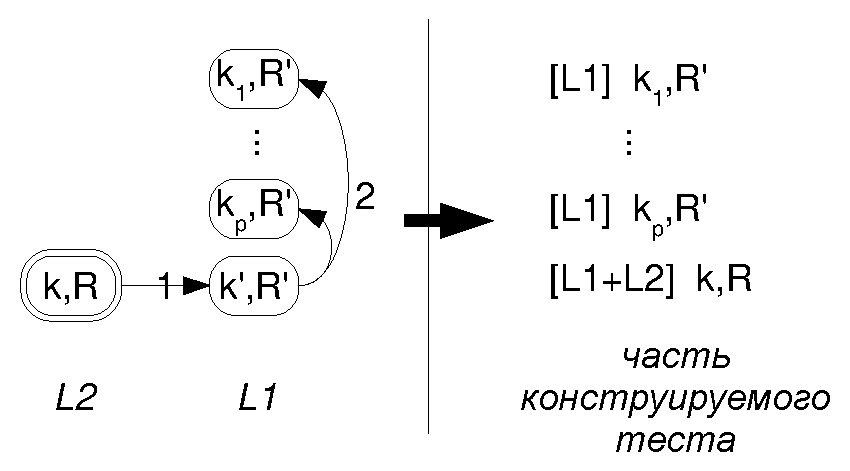
\includegraphics[width=0.6\textwidth]{2.theor/L1L2}
\caption{Конструирование обращения в кэш-память второго уровня вместе с
обращениями в кэш-память первого уровня}\label{fig:L1L2}
\end{figure}

Итак, по последовательности ключей и регионов для кэш-памяти первого уровня
инструкция составляется по только что приведенной схеме. С одним лишь
уточнением, что адрес должен быть таким, что при обращении по нему кэш-память
второго уровня не задействована. Теперь разберемся с последовательностью ключей
и регионов для кэш-памяти второго уровня. Рисунок~\ref{fig:L1L2} схематически
показывает, какие дополнительные инструкции надо построить для произвольного
обращения по ключу $k$ в регион $R$ кэш-памяти второго уровня. А именно, ключу
$k$ в регионе $R$ соответствует некоторый адрес, этому же адресу соответствуют и
некоторый ключ $k'$ в регионе $R'$ кэш-памяти первого уровня (стрелка с цифрой
1). Но надо еще обеспечить отсутствие этого ключа, иначе обращения в кэш-память
второго уровня не будет. Для этого надо сгенерировать небольшую
последовательность произвольных различных и не равных $k'$ ключей $k_1, k_2,
\dots, k_p$ и обратиться по ним в регион $R'$ кэш-памяти первого уровня без
затрагивания кэш-памяти второго уровня (значение числа $p$ зависит от стратегии
вытеснения).

%Рассмотрим один часто встречающийся случай кэширующих буферов,
%инициализация которого может вызывать трудности. Речь идет о
%кэш-памяти второго уровня. Зачастую кэш-память второго уровня не
%может быть инициализирована отдельно от остальных подсистем
%микропроцессора, обычно оно связано с изменением кэш-памяти первого
%уровня. Это создает дополнительные сложности при формулировании
%ограничений методом зеркальной генерации, поскольку инициализирующая
%последовательность должна подготавливать сразу два кэширующих буфера
%одновременно -- кэш-память первого уровня и кэш-память второго
%уровня. Кроме того, зачастую кэш-память второго уровня является
%совместной для хранения в ней данных и инструкций. Поэтому на
%инициализацию кэш-памяти второго уровня влияют и сами
%инициализирующие инструкции, и даже адрес расположения тестовой
%программы в памяти (от него зависит виртуальный адрес инструкций, а
%значит теги и индексы при обращении к кэш-памяти инструкций).
%
%Если принять дополнительное требование (и оно даст решение), что в
%кэш-памяти второго уровня наборы, используемые для доступа к
%инструкциям, не пересекаются с наборами, используемыми для доступа к
%данным, то генерируемые ограничения упрощаются (кэширование
%инструкций можно вообще не учитывать). С точки зрения зеркальной
%генерации это означает, что надо сформулировать требования на
%инициализирующую последовательность. Напомню, что одним из ключевых
%требований является произвольность начального состояния
%(содержимого) кэш-памяти.
%
%Предположим, что обращение к кэш-памяти второго уровня
%осуществляется при кэш-промахе в кэш-памяти первого уровня и
%кэш-память не является virtually indexed virtually
%tagged~\cite{HennessyPatterson3rd}. Для составления ограничений с
%использованием функций полезности необходимо знать, которые
%инструкции среди инициализирующей последовательности действительно
%обращаются в кэш-память второго уровня (иными словами, в каких
%инструкциях среди инициализирующей последовательности происходит
%кэш-промах при обращении к кэш-памяти первого уровня). Возможным
%решением было бы перебирать всевозможные распределения тестовых
%ситуаций в кэш-памяти первого уровня на элементах инициализирующей
%последовательности (с предварительной подготовкой этих тестовых
%ситуаций). Однако следующая лемма~\ref{special_initialization_L2}
%показывает, что для любого такого произвольного распределения
%тестовых ситуаций в кэш-памяти первого уровня существует решение со
%специальным распределением тестовых ситуаций. Это позволяет
%перебирать только такие специальные распределения тестовых ситуаций
%в кэш-памяти первого уровня. При этом вычислительная сложность
%процедуры поиска инициализирующей последовательности, дающей
%решение, изменяется от экспоненциальной от длины тестового шаблона к
%полиномиальной, что показывает лемма~\ref{max_k_h} (ее доказательство
%приведено в приложении~\ref{proofs}):
%\begin{lemma}[Верхняя оценка длины специальной инициализирующей
%последовательности для стратегии вытеснения \LRU]\label{max_k_h}\MaxUpperBoundLRU
%\end{lemma}
%\begin{sld}
%$$m = O(n)$$ где $m$ --- длина специальной инициализирующей
%последовательности, $n$ -- количество инструкций тестового шаблона.
%\end{sld}
%
%Для получения инициализирующей программы минимальной длины, можно
%применять сначала двоичный поиск суммы $k+h$ с применением
%дальнейшего поиска допустимых значений $k$ и $h$.